\documentclass[final]{sig-alternate-05-2015}

\usepackage{url}                  % format URLs
\usepackage{listings}          % format code
\lstset{
  mathescape, 
  language={C},
  basicstyle=\small
}
\usepackage{enumitem}      % adjust spacing in enums
\usepackage[colorlinks=true,allcolors=blue,breaklinks,draft=false]{hyperref}   
\usepackage{graphicx}
\usepackage{float}
\usepackage{subcaption}
\usepackage{xspace,framed}
\usepackage{colortbl}
\usepackage{calc}
\usepackage[dvipsnames]{xcolor}
\usepackage{amssymb,amsmath,amsfonts} 
\usepackage{mathtools}
\usepackage{microtype}

\usepackage{algorithm}
\usepackage{amsfonts}
\usepackage{multicol}
\usepackage{multirow}
\usepackage{tikz}
\usetikzlibrary{positioning, automata, shapes.arrows, calc, shapes, arrows}
\usetikzlibrary{patterns}
\usepackage[justification=centering]{caption}
\usepackage{stmaryrd}
\usepackage{hhline}
\usepackage{pifont}
\usepackage{longtable}
\usepackage{afterpage}
\usepackage{wasysym}
\usepackage[scaled]{helvet}

%\usetikzlibrary{decorations}
%\usetikzlibrary{decorations.pathmorphing}

\newcommand{\blue}[1]{{\color{blue}#1}}
\newcommand{\red}[1]{{\color{red}#1}}
\newcommand{\green}[1]{{\color{green}#1}}

\newtheorem{myassumption}{Assumption}
\newtheorem{mylemma}{Lemma}
\newtheorem{myprop}{Proposition}

%\renewcommand{\baselinestretch}{0.975}
\allowdisplaybreaks
\newcommand{\lcsay}[1]{{\color{Magenta} LC: {#1}}} 
\newcommand{\dcsay}[1]{{\color{purple} DC: {#1}}}
\newcommand{\dksay}[1]{{\color{blue} DK: {#1}}}  
\newcommand{\aasay}[1]{{\color{red} AA: {#1}}} 
\newcommand{\cdsay}[1]{{\color{Mahogany} CD: {#1}}} 
\newcommand{\pksay}[1]{{\color{RoyalBlue} PK: {#1}}} 
\newcommand{\ibsay}[1]{{\color{Sepia} IB: {#1}}} 

\newcommand{\param}[2]{\ensuremath{\langle{#1},{#2}\rangle}\xspace}
\newcommand{\xmark}{\ding{55}}
\newcommand{\tbmark}{\hspace{-1.2em}$^*$}


\begin{document}

% Copyright
\setcopyright{acmcopyright}

% DOI
\doi{}

% ISBN
\isbn{}

%
% --- Author Metadata here ---
%\conferenceinfo{WOODSTOCK}{'97 El Paso, Texas USA}
%\CopyrightYear{2007} % Allows default copyright year (20XX) to be over-ridden - IF NEED BE.
%\crdata{0-12345-67-8/90/01}  % Allows default copyright data (0-89791-88-6/97/05) to be over-ridden - IF NEED BE.
% --- End of Author Metadata ---

\title{
Sound and Automated Synthesis of Digital Stabilizing Controllers for Continuous Plants
%Counterexample-guided Synthesis of Closed-loop Digital Control Systems
}
%\subtitle{[Extended Abstract]
%\titlenote{A full version of this paper is available as
%\textit{Author's Guide to Preparing ACM SIG Proceedings Using
%\LaTeX$2_\epsilon$\ and BibTeX} at
%\texttt{www.acm.org/eaddress.htm}}}
%
% You need the command \numberofauthors to handle the 'placement
% and alignment' of the authors beneath the title.
%
% For aesthetic reasons, we recommend 'three authors at a time'
% i.e. three 'name/affiliation blocks' be placed beneath the title.
%
% NOTE: You are NOT restricted in how many 'rows' of
% "name/affiliations" may appear. We just ask that you restrict
% the number of 'columns' to three.
%
% Because of the available 'opening page real-estate'
% we ask you to refrain from putting more than six authors
% (two rows with three columns) beneath the article title.
% More than six makes the first-page appear very cluttered indeed.
%
% Use the \alignauthor commands to handle the names
% and affiliations for an 'aesthetic maximum' of six authors.
% Add names, affiliations, addresses for
% the seventh etc. author(s) as the argument for the
% \additionalauthors command.
% These 'additional authors' will be output/set for you
% without further effort on your part as the last section in
% the body of your article BEFORE References or any Appendices.

%\numberofauthors{8} %  in this sample file, there are a *total*
% of EIGHT authors. SIX appear on the 'first-page' (for formatting
% reasons) and the remaining two appear in the \additionalauthors section.
%
%% \author{
%% % You can go ahead and credit any number of authors here,
%% % e.g. one 'row of three' or two rows (consisting of one row of three
%% % and a second row of one, two or three).
%% %
%% % The command \alignauthor (no curly braces needed) should
%% % precede each author name, affiliation/snail-mail address and
%% % e-mail address. Additionally, tag each line of
%% % affiliation/address with \affaddr, and tag the
%% % e-mail address with \email.
%% %
%% % 1st. author
%% \alignauthor
%% Ben Trovato\titlenote{Dr.~Trovato insisted his name be first.}\\
%%        \affaddr{Institute for Clarity in Documentation}\\
%%        \affaddr{1932 Wallamaloo Lane}\\
%%        \affaddr{Wallamaloo, New Zealand}\\
%%        \email{trovato@corporation.com}
%% % 2nd. author
%% \alignauthor
%% G.K.M. Tobin\titlenote{The secretary disavows
%% any knowledge of this author's actions.}\\
%%        \affaddr{Institute for Clarity in Documentation}\\
%%        \affaddr{P.O. Box 1212}\\
%%        \affaddr{Dublin, Ohio 43017-6221}\\
%%        \email{webmaster@marysville-ohio.com}
%% }

\author{Alessandro Abate$^{1}$, Iury Bessa$^{2}$, Dario Cattaruzza$^{1}$, Lucas Cordeiro$^{1,2}$, \\ 
Cristina David$^{1}$, Pascal Kesseli$^{1}$ and Daniel Kroening$^{1}$
\and
$^{1}$\affaddr{University of Oxford, Oxford, United Kingdom} \\
$^{2}$\affaddr{Federal University of Amazonas, Manaus, Brazil}
}


\newcommand\tool{{\sf DSSynth}\xspace}

\maketitle

\begin{abstract}
%
Modern control is implemented with digital microcontrollers, which are
designed to work in an embedded environment, within a dynamical plant that
represents physical components.
%
We present a new algorithm based on counter\-example guided inductive
synthesis that automates the design of digital controllers that are
correct by construction.  The synthesis result is sound with respect to the
complete range of approximations, including time discretization,
quantization effects, and finite-precision arithmetic and their related
rounding errors.
%
We have implemented our new algorithm in a tool called \tool, and are able
to automatically generate stable controllers for a set of intricate plant
models taken from the literature within minutes.
%
\end{abstract}

%
%  Use this command to print the description
%
\printccsdesc

% We no longer use \terms command
%\terms{Theory}

\keywords{Control synthesis, CEGIS, finite word length, time sampling, quantization, interval analysis}

%%%%%%%%%%%%%%%%%%%%%%%%%%%%%%%%%%%%%%%%%%%%%%%%%%%%%%%%%%%%%%%%%%%%%%%%%%%%%%%%%%%%%%
\section{Introduction}

Modern implementations of embedded control systems have proliferated with the
availability of low-cost devices that can perform highly non-trivial control
tasks, with significant impact in numerous application areas such as
environmental control and robotics~\cite{astrom1997computer, Franklin15}.

Correct and sound control is non-trivial, however. The problem is exacerbated by
artefacts specific to digital control, such as the effects of
finite-precision arithmetic, time discretization, and quantization noise
introduced by A/D and D/A conversion.  Thus, the programming is a key
barrier to broad adoption of digital control, and requires considerable
expertise.

Beyond classical a-posteriori validation procedures in digital control,
there has been plenty of previous work aiming at \emph{verifying} a given
controller designed by the engineer.  Recent work can show the stability of
digital controllers with consideration of implementation aspects, i.e.,
fixed-point arithmetic and the word length used~\cite{Bessa16}.  The authors
of~\cite{Bessa16} exploit advances in bit-accurate verification of C
programs to obtain a verifier for software-implemented digital control.

By contrast, we leverage a very recent step-change in the scalability of
\emph{program synthesis}.  Program synthesis engines use a program
specification as the starting point, and subsequently generate a sequence of
candidate programs.  The candidate programs are iteratively refined to match
the specification more closely.  Program synthesizers that implement
Counter-Example Guided Inductive Synthesis (CEGIS)~\cite{sketch} are now
able to generate programs for highly non-trivial specifications with a very
high degree of automation.  Modern CEGIS engines combine automated testing,
genetic algorithms and SMT-based automated
reasoning~\cite{DBLP:conf/lpar/DavidKL15, DBLP:conf/cav/0001A14}.

By applying a state-of-the-art CEGIS engine we are now able to present a
tool that automatically \emph{generates} digital controllers for a given
continuous plant model that are correct by construction.  This approach
promises to reduce the cost and time of development of digital control
dramatically, and requires considerably less expertise than methodologies
driven by verification.  Specifically, we synthesize controllers for hybrid
closed-loop systems, i.e., software-implemented embedded controllers along
with a model of their physical environment (the plant), that are
\emph{stable}.  Due to the complexity of such systems, in this work we focus
on linear models with known configurations and perform parametric synthesis
of stabilizing digital controllers.

Our work addresses particularly challenging aspects of the control synthesis
problem.  We perform digital control synthesis over a hybrid model, where
the plant exhibits continuous behavior whereas the controller operates in
discrete time and over a quantized domain.  Inspired by a classical
approach~\cite{astrom1997computer}, we translate the problem into a single
digital domain.  Given our primary interest in stability despite
digitization effects, we have modeled a digital equivalent of the plant by
evaluating the effects of the quantizers (A/D and D/A converters) as time
discretization elements with quantization noise.  The resulting closed-loop
system is a program loop that operates on bit-vectors encoded using
fixed-point arithmetic with finite word length (FWL).  The deterministic
effects of the FWL and quantization errors are incorporated into the model
as an additive uncertainty, which is taken into account during the
CEGIS-based synthesis of the control software for the plant.

In summary, this paper makes the following original contributions.
%
\begin{itemize}

\item We design and implement an automatic approach in our tool \tool  
  for generating {\em correct-by-construction} digital controllers that is
  based on state-of-the-art inductive synthesis techniques.  Our application
  of program synthesis is non-trivial and requires addressing challenges
  specific to embedded control systems, such as the effects of quantizers
  and FWL.  In particular, we have found that a two-stage verification
  engine that continuously refines the precision of the fixed-point
  representation of the plant is key to the performance of our approach
  yielding, in most cases, a speed-up of at least two orders of magnitude
  over a conventional one-stage verification engine.

\item We provide experimental results showing that \tool is able to
  efficiently synthesize stable controllers for a set of intricate
  benchmarks taken from the literature: the median runtime for our benchmark
  set is $197$s, i.e., half of the controllers can be synthesized in less
  than five minutes.

%% \item We exploit a CEGIS-based approach that uses inductive synthesis
%% together with a bit-precise formal verification algorithm for synthesizing
%% correct-by-design robust digital controllers for non-fragile closed-loop
%% stability.

%% \item Experimental results with our synthesizer show that the
%% combination of interval arithmetic to represent the controller coefficients
%% and a two-stage verification approach to continuously refine precision
%% enables us to compute a parametric, sound solution for $14$ out of $15$
%% digital stabilizing controllers for a set of continuous and discrete plants
%% with parametric uncertainties.

\end{itemize}

%\begin{figure}
%\centering
%\resizebox{.35\textwidth}{!}{
% \begin{tikzpicture}[scale=0.3,-,>=stealth',shorten >=.2pt,auto,
%     semithick, initial text=, ampersand replacement=\&,]

%  \matrix[nodes={draw, fill=none, shape=rectangle, minimum height=.2cm, minimum width=.2cm, align=center}, row sep=.5cm, column sep=.5cm] {
%   \coordinate (aux0);
%   \& \node[circle] (circle) {}; 
%   \& \node[fill=yellow!20] (da) {{\sc D/A}}; 
%   \& \node[fill=yellow!20] (p) {{\sc P}};
%   \& \node[fill=yellow!20] (ad) {{\sc A/D}}; 
%   \& \coordinate (aux1);\\
%   \& \coordinate (aux3); 
%   \&
%   \&
%   \node[fill=yellow!20] (c) {C};
%   \& 
%   \& \coordinate (aux2);\\
%  };


%  \path[->] (aux0) edge (circle.west);
%  \path  
%   (circle.east) edge (da.west)
%   (da.east) edge (p.west)
%   (p.east) edge (ad.west)
%   (ad.east) edge (aux1.west)
%   (aux1.south) edge (aux2.north)
%   (aux2.west) edge (c.east)
%   (c.west) edge (aux3.east); 
%  \path[->]  (aux3.north) edge (circle.south);
% \end{tikzpicture}
%}
% \caption{Closed-Loop System. \label{fig:closed-system}}
%\end{figure}

We cover preliminaries on plant discretization, the verification of
closed-loop control systems, and stability in
Section~\ref{sec:preliminaries}.  Our core contribution is in
Section~\ref{sec:synthesis}: we present our CEGIS-based algorithm for
generating stable controllers for a given plant model.  Our experimental
setup and experimental results are given in Section~\ref{sec:experiments},
and we discuss how we extend the state-of-the-art beyond the existing
literature in Section~\ref{sec:related}. We conclude and describe future
work in Section~\ref{sec:conclusions}.

%%%%%%%%%%%%%%%%%%%%%%%%%%%%%%%%%%%%%%%%%%%%%%%%%%%%%%%%%%%%%%%%%%%%%%%%%%%%%%%%%%%%%%
\section{Preliminaries}\label{sec:preliminaries}

%\blue{Please insert a figure clearly distinguishing between continuous and discretised/quantised plant - a template is in a picture sent out by Lucas late last week. Please introduced signals on the plot. 

%Let us straighten the notations next. 
%We should have 
%\begin{itemize}
%\item 
%$G(s) = \frac{s^{M_G}b_{0}+s^{M_G-1}b_{1}+...+b_{M_G}}{s^{N_G}a_{0}+s^{N_G-1}a_{1}+...+a_{N_G}}$ -- this is the physical plant, which is focus of interest and to which we refer our specifications/properties 
%\item 
%$G(z, T) = \frac{\bar b_{0}+\bar b_{1}z^{-1}+...+\bar b_{M_G}z^{-M_G}}{\bar a_{0}+\bar a_{1}z^{-1}+...+\bar a_{N_G}z^{-N_G}}$ -- this is the time-discretised plant (notice the notation encompasses explicitly the sample time $T$; please write out explicitly the relationship between the $a_i$ and the $\bar a_i$ and likewise for the numerator's coefficients 
%(in particular, are the orders $M_G, N_G$ the same? 
%\item 
%we have $Y(z) = G(z,T) U(z)$; then, we introduce $\hat Y(z) \doteq Y(z) + \nu (z)$, so that 
%$$
%\frac{\hat Y(z)}{U(z)} = G(z,T) + \frac{\nu (z)}{U(z)} = G(z,T) + \Delta G_Q(z) \doteq \hat G(z) ,  
%$$ 
%where $\Delta G_Q(z)$ is an error term accounting for the quantization effects 
%\item 
%finally, we encompass the errors resulting from employing finite parameters representation, 
%which we encompass in a term $\Delta G_P(z)$: is this error additive, so that we would get to a 
%$$
%\tilde G(z) \doteq \hat G(z) + \Delta G_P(z) = G(z,T) + \Delta G_Q(z) + \Delta G_P(z)?  
%$$ 
%Dario, can you write it out explicitly? In other words, if 
%$$
%\hat G(z) = G(z,T) + \Delta G_Q(z) = \frac{\hat b_{0}+\hat b_{1}z^{-1}+...+\hat b_{M_G}z^{-M_G}}{\hat a_{0}+\hat a_{1}z^{-1}+...+\hat a_{N_G}z^{-N_G}},  
%$$ 
%then what is the explicit expression of 
%$$
%\tilde G(z) = \frac{\tilde b_{0}+\tilde b_{1}z^{-1}+...+\tilde b_{M_G}z^{-M_G}}{\tilde a_{0}+\tilde a_{1}z^{-1}+...+\tilde a_{N_G}z^{-N_G}}?
%$$
%(Notice that the orders $M_G, N_G$ need to be properly taken care of.)
%\item 
%Now, it's over the transfer function $\tilde G(z)$ that we want to synthesise the parameters of a template $C(z)$. 
%This controller's transfer function will be subject to the same quantization and precision limits as the plant's: 
%we need to argue that the way we do synthesis affects manipulation of quantities that relate to specific errors and be explicit about these. 
%\item[]
%\item 
%An additional source of error can be related to the fact that a plant transfer function, 
%per se a physical entity, is actually represented in a program imprecisely: 
%this would mean that $G(s)$ is actually 
%$$
%G^\ast (s) \doteq \frac{s^{M_G^\ast}b_{0}+s^{M_G^\ast-1}b_{1}+...+b_{M_G}}{s^{N_G^\ast}a_{0}+s^{N_G^\ast-1}a_{1}+...+a_{N_G}}, 
%$$ 
%which perhaps can indeed be re-written as $G^\ast (s) = G(s) + \Delta G_P(s)$? (This proof should come from that above.) 
%We should argue that this error is encompassed by the one derived above (or isn't it?). 
%\end{itemize}
%}

%------------------------------------
\subsection{Discretizing the Plant}
\label{ssec:SandH}
%------------------------------------

The digital controllers synthesized using the algorithm we present in this
paper are typically used in closed loops with continuous (physical) plants. 
Thus, the proposed approach has to consider dynamics of continuous parts of
the system (i.e., the plant) and of discrete parts (i.e., the digital
controller).  To obtain a joint model, we fully discretize the continuous
plant.  We briefly recall the standard foundations of this step.

We only consider transfer function models, and require a $z$-domain
transfer function $G(z)$ that captures all aspects of the continuous plant (with a
Laplace domain transfer function $G(s)$) and the sampling and hold process.
%Note that $G(z)$ is a discrete model of a physical, continuous
%plant, i.e., 
The continuous model of the plant must be discretized to obtain the corresponding 
%discrete equivalent 
coefficients of $G(z)$.
%via ZOH discretization.

%\red{[why do we discuss the ZOH at this point?]}

Among the discretization methods available in the
literature~\cite{Franklin15}, the zero-order hold (ZOH) discretization is
considered suitable for representing the sample and hold processes that are
typically employed in complex systems~\cite{istepanian2012digital}.  The ZOH
discretization models the exact effect of sampling and DAC interpolation
over the plant.

\begin{myassumption}
%
The sample and hold effects of the ADC and the ZOH of the DAC are synchronized,
i.e., there is no delay between sampling the plant output at ADC and
updating the DAC accordingly.  The DAC interpolator is an ideal ZOH. 
%
\end{myassumption}

\begin{mylemma}\cite{astrom1997computer}
%
Given a synchronized ZOH input and sample and hold output on the plant with
a sample time $T$ satisfying the Nyquist criterion, the discrete pulse
transfer function $G(z,T)$ is an exact z-domain representation of $G(s)$
that can be computed using the following formula:
%
\begin{equation}
\label{eq:pulsetf}
G(z,T) = %\mathcal{ZOH}\left\lbrace{G(s)}\right\rbrace =
(1-z^{-1})\mathcal{Z}\left\lbrace{\mathcal{L}^{-1}\left\lbrace{\frac{G(s)}{s}}\right\rbrace_{t=kT}}\right\rbrace.
\end{equation}
%
\end{mylemma}
%
For the sake of brevity, we will use the notation $G(z)$ to represent the
pulse transfer function.

Lemma~\ref{eq:pulsetf} ensures that the poles and zeros match under the
$\mathcal{Z}\left\lbrace{\mathcal{L}^{-1}\left\lbrace{\cdot}\right\rbrace_{t=kT}}\right\rbrace$
operations, and it includes the ZOH dynamics in the $(1-z^{-1})$ term, which
is sufficient for stability studies over $G(s)$.

%------------------------------------
\subsection{Verifying Closed-loop Control Systems}
\label{verifying-closed-loop-control-systems}
%------------------------------------

%\red{[This section and the next should be merged into a crisp section with the background on DSVerifier, if not included in previous work? 
%Please stick to the introduced notations. Please clarify what the function FWL does, compared to the general approximations introduced above.]}

%\red{Alessandro, I've made the changes as requested. Please let me know if this is good enough or if I made it too short}

%\textcolor{blue}{[IB: I'm proposing some changes in this section based on Alessandro's comments and trying to obtain a simpler and uniform notation.]}

CEGIS-based control synthesis requires a formal verifier to check whether a
candidate controller meets the requirements when combined with the plant. 
We use the Digital-System Verifier (DSVerifier)~\cite{IsmailBCFF15} for this
purpose.  It checks the stability of closed-loop control systems and
considers finite-word length (FWL) effects in the digital controller and
uncertainty parameters in the plant model (plant intervals)~\cite{Bessa16}. 
Let $C(z)$ be a digital controller and $G(z)$ be a plant model given as
%
\begin{align}
\small
\label{controller_plant_tf}
C(z)&=\frac{C_n(z)}{C_d(z)}=\frac{\beta_{0}+\beta_{1}z^{-1}+...+\beta_{M_C}z^{-M_C}}{\alpha_{0}+\alpha_{1}z^{-1}+...+\alpha_{N_C}z^{-N_C}}, \\
%\label{plant_tf}
G(z)&=\frac{G_n(z)}{G_d(z)}=\frac{b_{0}+b_{1}z^{-1}+...+b_{M_G}z^{-M_G}}{a_{0}+a_{1}z^{-1}+...+a_{N_G}z^{-N_G}}.
\end{align}
%
\noindent where $\vec{\beta}$ and $\vec{\alpha}$ are vectors containing the
controller's coefficients; similarly, $\vec{b}$ and $\vec{a}$ denote the
plant's coefficients; and $N_{(\cdot)}$ and $M_{(\cdot)}$ indicate the order
of the polynomial of the corresponding block.

Uncertainties in $G(z)$ may appear due to uncertainties in $G(s)$ (i.e.,
$\Delta_p{G}_n(s),\Delta_p{G}_d(s)$, which arise from tolerances/imprecision
in the original model), errors in the numeric calculations, or roundoffs in
the quantization.  These uncertainties are parametrically expressed by
additive terms, resulting in an uncertain model $\hat{G}(z)$, such that:
%
\begin{equation}
\hat{G}(z)=\frac{G_n(z)+\Delta G_n(z)}{G_d(z)+\Delta G_d(z)},
\end{equation}
%
which will be represented by the following transfer function:
%
\begin{equation}
\hat{G}(z)=\frac{\hat{b}_{0}+\hat{b}_{1}z^{-1}+...+\hat{b}_{M_G}z^{-M_G}}{\hat{a}_{0}+\hat{a}_{1}z^{-1}+...+\hat{a}_{N_G}z^{-N_G}} : N_G \geq M_G .
\end{equation}
%
Due to the nature of the methods we use for the stability check, we require
that the parametric errors in the plant have the same polynomial order as
the plant itself (all other errors described in this paper are ensured to
fulfill this property in our implementation).

In order to simplify the presentation, we employ a notation based on the
coefficients of the polynomials.  Let $\mathcal{P}^{N}$ be a polynomial
domain of order $N$. Let $P \in \mathcal{P}^{M,N}$ be a rational polynomial
$\frac{P_n}{P_d}$, where $P_n \in \mathcal{P}^{M}$ and $P_d \in \mathcal{P}^{N}$.  
For a vector of coefficients
%
\begin{equation}
\vec{P} \in \mathbb{R}^{N+M+2}=[n_{0}\ n_{1}\ \hdots \ n_{M}\ d_{0}\ d_{1}\ \hdots\ d_{N}\ ]^T
\label{eq:coefficients}
\end{equation}
%
and an uncertainty vector 
%
\begin{equation}
\Delta{\vec{P}}=[\Delta{n}_{0}\ \Delta{n}_{1}\ \hdots \ \Delta{n}_{M}\ \Delta{d}_{0}\ \Delta{d}_{1}\ \hdots\ \Delta{d}_{N}\ ]^T \; 
\label{eq:delta_coefficients}
\end{equation}
%
we write $\vec{\hat{G}}=\vec{G}+\Delta{\vec{G}}$.  In the following we will
either use the functions $G(z)$, $C(z)$ directly, or work over their
respective coefficients $\vec{G}$, $\vec{C}$ in vector form.

\begin{figure*}[htb]
\centering

\tikzset{add/.style n args={4}{
    minimum width=6mm,
    path picture={
        \draw[circle] 
            (path picture bounding box.south east) -- (path picture bounding box.north west)
            (path picture bounding box.south west) -- (path picture bounding box.north east);
        \node[draw=none] at ($(path picture bounding box.south)+(0,0.13)$)     {\small #1};
        \node[draw=none] at ($(path picture bounding box.west)+(0.13,0)$)      {\small #2};
        \node[draw=none] at ($(path picture bounding box.north)+(0,-0.13)$)    {\small #3};
        \node[draw=none] at ($(path picture bounding box.east)+(-0.13,0)$)     {\small #4};
        }
    }
 }

\resizebox{1.0\textwidth}{!}{
 \begin{tikzpicture}[scale=0.6,-,>=stealth',shorten >=.2pt,auto,
     semithick, initial text=, ampersand replacement=\&,]

  \matrix[nodes={draw, fill=none, shape=rectangle, minimum height=.2cm, minimum width=.2cm, align=center}, row sep=.6cm, column sep=.6cm] {
    \node[draw=none] (r) {$R(z)$};
%   \& \coordinate (aux0);
   \& \node[circle,add={-}{+}{}{}] (circle) {};
   \node[draw=none] (ez) at ([xshift=1cm,yshift=.15cm]circle)  {$e(z)$};
   \& \node[rectangle,draw,
	minimum width=1cm,
	minimum height=1cm,
        label=\textbf{Controller}] (cz) {{\sc C(z)}};
   \node[draw=none] (ud) at ([xshift=1cm,yshift=.15cm]cz)  {$U(z)$};
     
   \& complexnode/.pic={ 
      \node[rectangle,draw,
	minimum width=3cm,
	minimum height=1.6cm,
	label=\textbf{DAC},] (dac) {};
     \node[circle,add={}{+}{+}{},fill=gray!20] (q2) at ([xshift=-.65cm]dac.center) {};
     \node[draw=none] (q2t)  at ([xshift=-.65cm,yshift=-.65cm]dac.center) {{\sc Q2}};
     \node[draw=none] (v2)  at ([xshift=-.65cm,yshift=1.5cm]dac.center) {$\nu_2(z)$};
     \node[fill=gray!20] (zoh) at ([xshift=.65cm]dac.center) {{\sc ZOH}};}   
   \& \node[rectangle,draw,
	minimum width=1cm,
	minimum height=1cm,
        label=\textbf{Plant}] (gs) {{\sc $\hat{G}(s)$}};
   \node[draw=none] (ud) at ([xshift=-2cm,yshift=.15cm]gs)  {$U(s)$};
   \node[draw=none] (y) at ([xshift=2cm,yshift=.15cm]gs)  {$Y(s)$};
   \& complexnode/.pic={ 
     \node[rectangle,draw,
	minimum width=4cm,
	minimum height=1.6cm,
	label=\textbf{ADC},] (adc) {};
   \draw[] ([xshift=-1cm]adc.center) -- ++(0.5,0.2cm);
   \coordinate (switch1) at ([xshift=-1cm]adc.center);
   \coordinate (switch2) at ([xshift=-0.4cm]adc.center);
   \node[circle,add={}{+}{+}{},fill=gray!20] (q1) at ([xshift=1cm]adc.center) {};} 
     \node[draw=none] (q2t)  at ([xshift=1cm,yshift=-.65cm]adc.center) {{\sc Q1}};
   \node[draw=none] (v1)  at ([xshift=1cm,yshift=1.5cm]adc.center) {$\nu_1(z)$};
   \& \coordinate (aux1);
   \& \node[draw=none] (yz) {$\hat{Y}(z)$};\\
   \& \coordinate (aux3); 
   \&
   \&
   \& 
   \& 
   \& \coordinate (aux2);\\
  };


  \path[->] (v1) edge (q1.north);
  \path[->] (v2) edge (q2.north);
  \path[->] (r) edge (circle.west);
  \path[->] (aux1) edge (yz);
  \path  
   (circle.east) edge (cz)
   (cz.east) edge (q2.west)
   (q2.east) edge (zoh.west)
   (zoh.east) edge (gs.west)
   (switch2) edge (q1.west)
   (q1.east) edge (aux1.west)
   (gs.east) edge (switch1.west)
   (aux1.south) edge (aux2.north)
   (aux2.west) edge (aux3.east); 
  \path[->]  (aux3.north) edge (circle.south);
 \end{tikzpicture}
}
 \caption{Closed-loop digital control system\label{fig:sampledsystem}}
\end{figure*}

%\begin{equation}
%\Delta{\vec{p}}=\begin{bmatrix}
%\hat{b_{0}} - b_{0}\\
%\hat{b_{1}} - b_{1}\\
%\vdots \\
%\hat{b}_{M_G} - b_{M_{G}}\\
%\hat{a_{0}} - a_{0}\\
%\hat{a_{1}} - a_{1}\\
%\vdots\\
%\hat{a}_{N_G} - a_{N_{G}}\\
%\end{bmatrix}=\begin{bmatrix}
%\vec{\hat{b}}\\
%\vec{\hat{a}}
%\end{bmatrix}-\begin{bmatrix}
%\vec{b}\\
%\vec{a}
%\end{bmatrix}
%\label{eq:uncertainty}
%\end{equation}

A typical digital control system with a continuous plant and a discrete
controller is illustrated in Figure~\ref{fig:sampledsystem}.  The DAC and
ADC converters introduce quantization errors which are modeled as noises
$\nu_{1}(z)$ and $\nu_{2}(z)$, $G(s)$ is the continuous-time plant model
with parametric additive uncertainty $\Delta_p{G}_n(s)$ and
$\Delta_p{G}_d(s)$, $R(z)$ is the reference signal, $U(z)$ is the control
signal, and $\hat{Y}(z)$ is the output signal affected by the noises and
uncertainties in the closed-loop system.
%
%
%
The ADC and DAC may be abstracted by transforming the closed-loop system in
Figure~\ref{fig:sampledsystem} into the digital system in 
Figure~\ref{fig:digsystem1}, where the parametric uncertainties are
represented by~$\Delta_p \vec{G}$
%
%=\mathcal{Z}\left\lbrace{G_{P}(s)}\right\rbrace$
%
and the entire effect of $\nu_{1}$ and $\nu_{2}$ in the output $Y(z)$ is
represented as an additive output noise~$\nu(z)$. 
%, thus
%$\hat{Y}(z)=Y(z)+\nu(z)$.  The measurement noise $\nu(k)$ is enough for
%represent both quantization noises ($\nu_{1}$ and $\nu_{2}$) what can be
%obtained reorganizing the equations~\ref{eq:outputfunctions}:
%%
%\begin{equation}
%\label{eq:outputfunctions2}
%\hat{Y}(z)=H_{1}R(z)+H_{1}\nu_{1}(z)+H_{2}(z)\nu_{2}(z),
%\end{equation}
%%
%where $H_{1}R(z)$ is exactly equal to $Y(z)$ without quantization noise effects, thus:
%%
%\begin{equation}
%\nu(z)=H_{1}\nu_{1}(z)+H_{2}(z)\nu_{2}(z).
%\end{equation}

%The system in equation~\ref{controller_plant_tf} (disregarding the $\Delta{G}_{P}(z)$ may be represented by the following difference equation model:
%\begin{equation}
%\begin{split}
%y(k)=-a_{1}y(k-1)-a_{2}y(k-2)-\cdots - a_{N}y(k-N)\\
%+b_{0}u(k)+b_{1}u(k-1)+b_{2}u(k-2)+\cdots+b_{M}u(k-M),
%\end{split}
%\end{equation}
%and consequently $\hat{y}(k)$ may be represented by the following difference equation:
%\begin{equation}
%\label{eq:differencewithnoise}
%\begin{split}
%\hat{y}(k)=-a_{1}y(k-1)-a_{2}y(k-2)-\cdots - a_{N_{G}}y(k-N_{G})\\
%+b_{0}u(k)+b_{1}u(k-1)+b_{2}u(k-2)+\cdots+b_{M_{G}}u(k-M_{G})+\nu(k).
%\end{split}
%\end{equation}
%
%The z-transform of~\eqref{eq:differencewithnoise} is:
%\begin{equation}
%\begin{split}
%\hat{Y}(z)=(-a_{1}z^{-1}-a_{2}z^{-2}-\cdots-a_{N_{G}}z^{-N_{G}})Y(z)\\
%+(b_{0}+b_{1}z^{-1}+b_{2}z^{-2}+\cdots+b_{M_{G}}z^{-M_{G}})U(z)+\nu(z),
%\end{split}
%\end{equation}
%dividing both sides by $U(z)$, it is equivalent to:
%\begin{equation}
%\frac{\hat{Y}(z)}{U(z)}=[1-D_{G}(z)]G(z)+U(z)D_{G}(z)+\frac{\nu(z)}{U(z)}=G(z)+\Delta{G}_{Q}(z),
%\end{equation}

%Considering the quantization noise $\nu(k)$ as an output error in discrete plant model, we may represent it as an additive noise in the plant output $y(k)$ resulting in the noisy output $\hat{y}(k)$:
%\begin{equation}
%
%\end{equation}

\begin{figure}[ht]
\centering
\tikzset{add/.style n args={4}{
    minimum width=6mm,
    path picture={
        \draw[circle] 
            (path picture bounding box.south east) -- (path picture bounding box.north west)
            (path picture bounding box.south west) -- (path picture bounding box.north east);
        \node[draw=none] at ($(path picture bounding box.south)+(0,0.13)$)     {\small #1};
        \node[draw=none] at ($(path picture bounding box.west)+(0.13,0)$)      {\small #2};
        \node[draw=none] at ($(path picture bounding box.north)+(0,-0.13)$)    {\small #3};
        \node[draw=none] at ($(path picture bounding box.east)+(-0.13,0)$)     {\small #4};
        }
    }
 }

\resizebox{.48\textwidth}{!}{
 \begin{tikzpicture}[scale=0.3,-,>=stealth',shorten >=.2pt,auto,
     semithick, initial text=, ampersand replacement=\&,]

  \matrix[nodes={draw, fill=none, shape=rectangle, minimum height=.2cm, minimum width=.2cm, align=center}, row sep=.6cm, column sep=.3cm] {
    \node[draw=none] (r) {$R(z)$};
%   \& \coordinate (aux0);
   \& \node[circle,add={-}{+}{}{}] (circle) {};
   \node[draw=none] (ez) at ([xshift=1cm,yshift=.15cm]circle)  {$e(z)$};
   \& \node[rectangle,draw,
	minimum width=1cm,
	minimum height=1cm,
        label=\textbf{Controller}] (cz) {{\sc C(z)}};
   \node[draw=none] (ud) at ([xshift=1cm,yshift=.15cm]cz)  {$U(z)$};
   \& \node[rectangle,draw,
	minimum width=1cm,
	minimum height=1cm,
        label=\textbf{Plant}] (gs) {{\sc $\hat{G}(z)$}};
   \node[draw=none] (y) at ([xshift=2cm,yshift=.15cm]gs)  {$Y(z)$};

   \& \node[circle,add={}{+}{+}{}] (circle2) {};
%   \node[draw=none] (tyz) at ([xshift=-1cm,yshift=.15cm]circle2)  {$Y(z)$};
   \node[draw=none] (nu) at ([yshift=1cm]circle2)  {$\nu(z)$};
   \& \coordinate (aux1);
   \& \node[draw=none] (yz) {$\tilde Y(z)$};\\
   \& \coordinate (aux3); 
   \&
   \& 
   \& 
   \& \coordinate (aux2);\\
  };


%  \path[->] (v1) edge (q1.north);
%  \path[->] (v2) edge (q2.north);
  \path[->] (r) edge (circle.west);
  \path[->] (nu) edge (circle2.north);
  \path[->] (aux1) edge (yz);
  \path  
   (circle.east) edge (cz)
   (cz.east) edge (gs.west)
   (gs.east) edge (circle2.west)
   (circle2.east) edge (aux1.west)
   (aux1.south) edge (aux2.north)
   (aux2.west) edge (aux3.east); 
  \path[->]  (aux3.north) edge (circle.south);
 \end{tikzpicture}
}
\caption{System equivalent to the system in Figure~\ref{fig:sampledsystem} 
\label{fig:digsystem1}}
\end{figure}

%
In Figure~\ref{fig:digsystem1}, two sources of uncertainty are illustrated:
parametric uncertainties related to modeling errors, and uncertainties
introduced by quantizations in sampling and holding process, i.e., ADC and
DAC conversions.  Assuming linearity and independence between these sources,
the uncertain model may be rewritten as a vector of coefficients in the
z-domain using equations (\ref{eq:coefficients}) and
(\ref{eq:delta_coefficients})
%
\begin{equation}
\label{eq:complete_unc_model}
\vec{\hat{G}}=\vec{G}+\Delta_p \vec{G}+\Delta_q \vec{G},
\end{equation}
%
where $\Delta_p \vec{G}$ is the term that corresponds to the parametric
uncertainties and $\Delta_q \vec{G}$ is the term that reflects the
quantization effects on the plant model.

%\red{[next figure is a bit unnecessary, does not ad much to the previous one.]} Figure~\ref{fig:digsystem2} shows the digital closed loop systems with $\Delta G_{P}(z)$ and $\Delta G_{Q}(z)$.


%\begin{figure}[ht]
%\centering
%
%\tikzset{add/.style n args={4}{
%    minimum width=6mm,
%    path picture={
%        \draw[circle] 
%            (path picture bounding box.south east) -- (path picture bounding box.north west)
%            (path picture bounding box.south west) -- (path picture bounding box.north east);
%        \node[draw=none] at ($(path picture bounding box.south)+(0,0.13)$)     {\small #1};
%        \node[draw=none] at ($(path picture bounding box.west)+(0.13,0)$)      {\small #2};
%        \node[draw=none] at ($(path picture bounding box.north)+(0,-0.13)$)    {\small #3};
%        \node[draw=none] at ($(path picture bounding box.east)+(-0.13,0)$)     {\small #4};
%        }
%    }
% }
%
%\resizebox{.5\textwidth}{!}{
% \begin{tikzpicture}[scale=0.3,-,>=stealth',shorten >=.2pt,auto,
%     semithick, initial text=, ampersand replacement=\&,]
%
%  \matrix[nodes={draw, fill=none, shape=rectangle, minimum height=.2cm, minimum width=.2cm, align=center}, row sep=.6cm, column sep=.3cm] {
%  %
%	\& 
%	\&
%	\& \coordinate (aux7); 
%	\& \node[rectangle,draw,
%	minimum width=1cm,
%	minimum height=1cm] (deltag2) {{\sc $\Delta G_{Q}(z)$}};
%	\& \coordinate (aux8);\\
%    \node[draw=none] (r) {$R(z)$};
%%   \& \coordinate (aux0);
%   \& \node[circle,add={-}{+}{}{}] (circle) {};
%   \node[draw=none] (ez) at ([xshift=1cm,yshift=.15cm]circle)  {$e(z)$};
%   \& \node[rectangle,draw,
%	minimum width=1cm,
%	minimum height=1cm,
%        label=\textbf{Controller}] (cz) {{\sc C(z)}};
%   \node[draw=none] (ud) at ([xshift=1cm,yshift=.15cm]cz)  {$U(z)$};
%   \& \coordinate (aux4);
%   \& \node[rectangle,draw,
%	minimum width=1cm,
%	minimum height=1cm,
%        label=\textbf{Plant}] (gs) {{\sc G(z)}};
%   \node[draw=none] (y) at ([xshift=1cm,yshift=.15cm]gs)  {$Y(z)$};
%   \& \node[circle,add={+}{+}{+}{}] (circle2) {};
%%   \node[draw=none] (tyz) at ([xshift=-1cm,yshift=.15cm]circle2)  {$Y(z)$};
%%   \node[draw=none] (nu) at ([yshift=1cm]circle2)  {$\nu(z)$};
%   \& \coordinate (aux1);
%   \& \node[draw=none] (yz) {$\hat{Y}(z)$};\\
%   \& 
%   \&
%   \& \coordinate (aux5); 
%   \& \node[rectangle,draw,
%	minimum width=1cm,
%	minimum height=1cm] (deltag) {{\sc $\Delta G_{P}(z)$}};
%   \& \coordinate (aux6);\\
%   \& \coordinate (aux3); 
%   \&
%   \& 
%   \& 
%   \&
%   \& \coordinate (aux2);\\
%  };
%
%
%%  \path[->] (v1) edge (q1.north);
%%  \path[->] (v2) edge (q2.north);
%  \path[->] (r) edge (circle.west);
%%  \path[->] (nu) edge (circle2.north);
%  \path[->] (aux1) edge (yz);
%  \path  
%   (aux4.north) edge (aux5.south)
%   (aux4.north) edge (aux7.south)
%   (aux5.east) edge (deltag.west)
%   (aux7.east) edge (deltag2.west)
%   (deltag.east) edge (aux6.west)
%   (deltag2.east) edge (aux8.west)
%   (circle.east) edge (cz)
%   (cz.east) edge (gs.west)
%   (circle2.east) edge (aux1.west)
%   (aux1.south) edge (aux2.north)
%   (aux2.west) edge (aux3.east); 
%  \path[->] (aux8.south) edge (circle2.north); 
%  \path[->] (aux6.south) edge (circle2.south);
%  \path[->] (gs.east) edge (circle2.west);
%  \path[->] (aux3.north) edge (circle.south);
% \end{tikzpicture}
%}
% \caption{Digital system with additive uncertainties $\Delta G_{P}(z)$ and $\Delta G_{Q}(z)$. \label{fig:digsystem2}}
%\end{figure}

%\textcolor{blue}{[IB: I propose to exchange the following paragraphs by the previous blue]}

%\textcolor{green}{DC: I believe Alessandro wanted to be more specific about the nature of the modelling error which is why I was trying to explain it. In this case I believe there are also two separate sources for $\Delta{G}_p(z)$. The first is $\Delta{G}_p(s)$ (which is basically a known tolerance that may come from G(t)), while the second is the error introduced by the calculations in the $\mathcal{Z}$ transform. Alessandro, do you want to address this second term (possibly as explained below) or just leave the blue section as is?}


%Since $G(z)$ is an approximation of $G(s)$ we introduce an error term caused during its calculation as $\Delta{G}_P$
%
%%
%\begin{align}
%\small
%\label{parametric_plant_tf}
%\hat{G}(z)&=\frac{(b_{0}+\Delta_p b_{0}) +...+(b_{M_G}+\Delta_p b_{M_G})z^{-M_G}}{(a_{0}+\Delta_p a_{0})+...+(a_{N_G}+\Delta_p a_{N_G})z^{-N_G}} \nonumber \\
%&=G(z)+\Delta{G}_P(z).
%\end{align}
%%
%Note that $\Delta{G}_P$ is undefined and upper bound by a user defined
%value such that $\hat{G}(z)$ corresponds to the set of
%possible polynomial forms of $G(z, T)$ that overapproximate $G(s)$.
%This calculation is performed outside of the scope of this work since it depends on the nature of the tool used to obtain the $\mathcal{Z}$ form. The error comes from the bounded horizon and mathematical precision used to calculate the $\mathcal{Z}$ transform, which will be tool and user dependent.
%\red{[The previous statement is confusing and I must disagree here: I want hard error bounds on a specific value of T.]}
%\green{[You are correct. It was absolutely wrong. Hopefully this explanation is clear. We use MATLAB, but still don't know the details of their implementation, so I don't have hard data on how this error is calculated.}

Since the controller is implemented using a FWL, $C(z)$ also suffers
disturbances from the FWL effects, with roundoffs in coefficients that may
change the closed-loop poles and zeros position, and consequently affect its
stability, as argued in~\cite{Bessa16}.

Let $\hat{C}(z)$ be the transfer function of the digital controller
represented using this FWL with integer size $I$ and fractional size~$F$. 
We shall denote the FWL domain of coefficients as $\mathbb{R}\langle I,F
\rangle$
%
%Since the controller is implemented in the $\mathbb{R}\langle I,F \rangle$ 
%domain, {\it i.e.} a Fixed-Point Finite Word Length with integer size $I$ and fractional
%size $F$, we shall denote this domain as $\mathbb{R}\langle I,F \rangle$ 
%
and assume that there exists a function
$\mathit{FWL}_n[\cdot]:\mathcal{P}^{n}\rightarrow \mathcal{P}^{n}\langle I,F \rangle$,
which applies the FWL effects to a polynomial, with an equivalent $\mathit{FWL}_{n,m}[\cdot]:\mathcal{P}^{n,m}\rightarrow \mathcal{P}^{n,m}\langle I,F \rangle$ that applies the same effect to a ratio of polynomials, where
$\mathcal{P}^{n}$ is the
space of polynomials of $n$-th order, $\mathcal{P}^{n}\langle I,F
\rangle$ is the space of polynomials with coefficients in
$\mathbb{R}\langle I,F \rangle$, and $\mathcal{P}^{n,m}$,  $\mathcal{P}^{n,m}\langle I,F
\rangle$ are their rational equivalent.

Thus, the perturbed controller model $\hat{C}(z)$ may be obtained from the
original model $C(z)=\frac{C_{n}(z)}{C_{d}(z)}$ as follows:
%
\begin{equation}
\hat{C}(z)=\mathit{FWL}_{M_C,N_C}[C(z)]=\frac{\mathit{FWL}_{M_C}[C_n(z)]}{\mathit{FWL}_{N_C}[C_d(z)]}.
\end{equation}
%
In the case of a synthesized controller, because the synthesis is performed
using FWL, $\hat{C}(z) \equiv C(z)$.

%\textcolor{blue}{[IB: And I propose to exchange the remaining paragraphs by the previous blue]}
%
%\textcolor{green}{[DC: I changed it to a separate section to differentiate the effects, so we should keep both]}

%------------------------------------
\subsection{Stability under FWL and Noise}
\label{sec:stability}
%------------------------------------

Correct synthesis of the digital controller requires consideration of the
effect of FWL on the controller and quantization noises in the closed loop
system.  Let the quantizer $Q1$ be the source of a white noise $\nu_{1}$ and
$Q2$ be the source of a white noise $\nu_{2}$.  The following equation
models the system in Figure~\ref{fig:sampledsystem}, encompassing the
parametric uncertainties $\Delta \vec{G}$ and the FWL effects on
the controller ($\hat{C}(z)$):
%
\begin{equation}
\hat{Y}(z)=\hat{C}(z)\hat{G}(z)[R(z)+\nu_{1}(z)]+\nu_{2}(z)\hat{G}(z)-\hat{Y}(z)\hat{C}(z)\hat{G}(z),
\end{equation}
%
The above can be rewritten as follows:
%
\begin{equation}
\label{eq:outputfunctions}
\hat{Y}(z)=H_{1}[R(z)+\nu_{1}(z)]+H_{2}(z)\nu_{2}(z),
\end{equation}
%
where
%
\begin{equation}
H_{1}=\frac{\hat{C}(z)\hat{G}(z)}{1+\hat{C}(z)\hat{G}(z)},
\end{equation}
%
and
%
\begin{equation}
H_{2}=\frac{\hat{G}(z)}{1+\hat{C}(z)\hat{G}(z)}.
\end{equation}

\begin{myassumption}
\label{whitenoise}
%
The quantization noises $\nu_{1}$ (from $Q1$) and $\nu_{2}$ (from $Q2$) are
uncorrelated white noises and their amplitudes are always bounded by the
half of quantization step~\cite{astrom1997computer}, i.e., $\vert \nu_{1}
\vert \leq \frac{q_{1}}{2}$ and $\vert \nu_{2} \vert \leq \frac{q_{2}}{2}$,
where $q_{1}$ and $q_{2}$, respectively, are the quantization steps of ADC
and DAC.
% 
\end{myassumption}

%\begin{mylemma}
%\label{lemma:variance}
%%
%In particular, Widrow \cite{widrow1956} models the quantization noise as a
%Gaussian model in which the second moment (variance) of the probability
%density function (PDF) of the quantization noise is given by
%%
%\begin{equation}
%\label{eq:variancelemma}
%\sigma_{Q}^{2}=\frac{q^{2}}{12},
%\end{equation}
%where $q$ is the step size of quantiser. (Proof is on \cite{widrow1956})
%\end{mylemma}
%
%\begin{mylemma}
%\label{lemma:boundednoise}
%%
%The power spectral density of the quantization noise (supposed white)
%$S_{\nu}(z)$ is bounded and may be computed through the z-transform of
%autocorrelation function of $\nu(k)$, thus:
%%
%\begin{equation}
%S_{\nu}(z)= \sigma_{Q}^{2}=\frac{q^{2}}{12}.
%\end{equation}
%\end{mylemma}
%
%\begin{proof}
%%
%Considering $\nu(k)$ a random process, where $\nu(k)$ is independent from
%$\nu(k+i)$ for every integer $k\neq 0$.  The autocorrelation function of
%$\nu(k)$, {\it i.e.} $R_{\nu\nu}(\tau)$ may be computed as follows:
%%
%\begin{equation}
%R_{\nu\nu}(\tau)=E[\nu(t+\tau)\nu(t)]=\sigma_{Q}^{2}\cdot \delta(\tau),
%\end{equation}
%%
%where $\delta(\tau)$ is the Dirac delta function at delay time $\tau$.
%
%By definition~\cite{poularikas2000transforms}, the power spectral density of
%$\nu(k)$ is the z-transform of $R_{\nu\nu}(\tau)$, thus
%%
%\begin{equation}
%S_{\nu}(z)=  \sum\limits_{k=-\infty}^{\infty}{R_{\nu\nu}(k)z^{-k}} = \sigma_{Q}^{2},
%\end{equation}
%considering the Lemma~\ref{lemma:variance}:
%\begin{equation}
%S_{\nu}(z)=  \frac{q^{2}}{12}.
%\end{equation}
%\end{proof}
%
%Finally, the quantization noise spectrum may be considered a energy-bounded
%(Lemma~\ref{lemma:boundednoise}), and consequently the Parseval's theorem
%ensures that the quantization noise is also energy-bounded in time-domain. 
%Thus $\hat{Y}(z)$ will be bounded and the closed-loop system stable if the
%conditions in Lemma~\ref{lemma:eq_int_stab} are followed.

%\red{[Add remark on bound (q/2) for signal. We need a bounded signal to be able to leverage BIBO stability results. ]}

A discrete-time linear system is said to be Bounded-Input and Bounded-Output
(BIBO) stable if and only if every pole of its transfer function lies inside
the unit circle \cite{Astrom08}.  Analyzing Eq.~\eqref{eq:outputfunctions},
the following proposition gives necessary conditions for BIBO stability of
the closed-loop system in Figure~\ref{fig:sampledsystem}, since the
exogenous signals $R(z)$, $\nu_{1}$, and $\nu_{2}$ are bounded.

\begin{myprop}{\cite{fadali,Bessa16}}
\label{prop:eq_int_stab} 
%
Consider a feedback closed-loop control system as given in
Figure~\ref{fig:sampledsystem} with a FWL implementation of the digital
controller $\hat{C}(z) =\mathit{FWL}_{M_C,N_C}[C(z)]$ and uncertain discrete
model of the plant
%
$$\hat{G}(z) =\frac{\hat{G}_n(z)}{\hat{G}_d(z)}: \vec{\hat{G}}=\vec{G}+\Delta_p \vec{G}+\Delta_q
\vec{G} \text{\quad(from~\ref{eq:coefficients},\ref{eq:delta_coefficients})}$$
%
Then $\hat{G}(z)$ is BIBO-stable if and only if:
%
\begin{itemize}
\item  the roots of characteristic polynomial $S(z)$ are inside the open unit circle, where $S(z)$ is:
\begin{equation}
\label{eq:internal_stab_lemma}
S(z)=\mathit{FWL}_{M_C}[C_n(z)]\hat{G}_n(z)+\mathit{FWL}_{N_C}[C_d(z)]\hat{G}_d(z);
\end{equation}
\item the direct loop product $\mathit{FWL}_{M_C,N_C}[C(z)]\cdot \hat{G}(z)$ has no pole-zero cancellation on or outside the unit circle.
\end{itemize}
\end{myprop}

Proposition~\ref{prop:eq_int_stab} provides the necessary conditions for the
digital controller to stabilize the closed-loop system, considering plant
parametric uncertainties (i.e., $\Delta_p \vec{G}$), quantization noises
($\nu_{1}$ and $\nu_{2}$) and FWL effects in the control software.  Notice
that the model for plant uncertainty due to quantization noise (i.e.,
$\Delta_q \vec{G}$) may be disregarded if the conditions on
Proposition~\ref{prop:eq_int_stab} are satisfied and if the quantization
noise is bounded.  The boundedness of the quantization noise comes from
Assumption~\ref{whitenoise}.

%\red{[first: lemmae precede theorems. ]}

% Let $\tilde C(z)$ and $\tilde G(z)$ be the transfer functions represented
% using Fixed-Point bit vectors with integer size $I_p$ and fractional
% size $F_p$, whose domain is $\mathbb{R}\langle I_p,F_p \rangle \supseteq \mathbb{R}\langle I,F \rangle$.
% %
% \begin{align}
% \small
% \label{digital_controller_plant_tf}
% \tilde C(z)&=\frac{\tilde \beta_{0}+\tilde \beta_{1}z^{-1}+...+\tilde \beta_{M_C}z^{-M_C}}{\tilde \alpha_{0}+\tilde \alpha_{1}z^{-1}+...+\tilde \alpha_{N_C}z^{-N_C}}, \\
% %\label{plant_tf}
% \tilde G(z)&=\frac{\tilde b_{0}+\tilde b_{1}z^{-1}+...+\tilde b_{M_G}z^{-M_G}}{\tilde a_{0}+\tilde a_{1}z^{-1}+...+\tilde a_{N_G}z^{-N_G}}.
% \end{align}
 
% Since the controller is synthesized in the $\mathbb{R}\langle I,F \rangle$
% domain,
% %
%  $$\forall i \leq N_C, j \leq M_C\ \  \tilde \beta_{i} \equiv \beta_{i} \wedge \tilde \alpha_{j} \equiv \alpha_{j} \Leftrightarrow \tilde C(z) \equiv C(z)$$

% Two approaches have been taken to synthesise a stable controller based on this model.
% The first uses interval arithmetic, representing the coefficients $[{c}_i-\Delta_p{c}_i-\Delta_b{c}_i\ ,\ {c}_i+\Delta_p{c}_i-\Delta_b{c}_i+(2^{-F_p})]$  

% \cdsay{Dario, what coefficients are these?}

% and rounding operations outwards during the process. This results in a tighter calculation of the error at the cost of performance.

%, thus supporting this assumption.

%------------------------------------
%\subsection{Using Fixed Point Arithmetic for verification}
%\label{fixedpoint_verification}
%------------------------------------



%%%%%%%%%%%%%%%%%%%%%%%%%%%%%%%%%%%%%%%%%%%%%%%%%%%%%%%%%%%%%%%%%%%%%%%%%%%%%%%%%%%%%%
\section{Automated Program Synthesis \\ for Digital
Control}\label{sec:synthesis}

%------------------------------------
\subsection{Overview of the Synthesis Process}
\label{verification-flow}
%------------------------------------

In order to synthesize closed-loop digital control systems, we use a program
synthesis engine.  Our program synthesizer implements Counter-Example Guided
Inductive Synthesis (CEGIS)~\cite{sketch}.  We start by presenting its
general architecture followed by describing the parts specific to
closed-loop control systems.  A high-level view of the synthesis process is
given in Figure~\ref{DSSynth_process}.  Steps $1$ to $3$ are performed by
the user and Steps~A to D are automatically performed by our tool for
Digital Systems Synthesis, named \tool.
%
%, which accepts the
%digital controller transfer functions together with the plant model.  For
%any digital controller, implementation details should be provided ({\it
%e.g.}, number of bits, realization, and sample time).

\begin{figure*}[t]
\centering
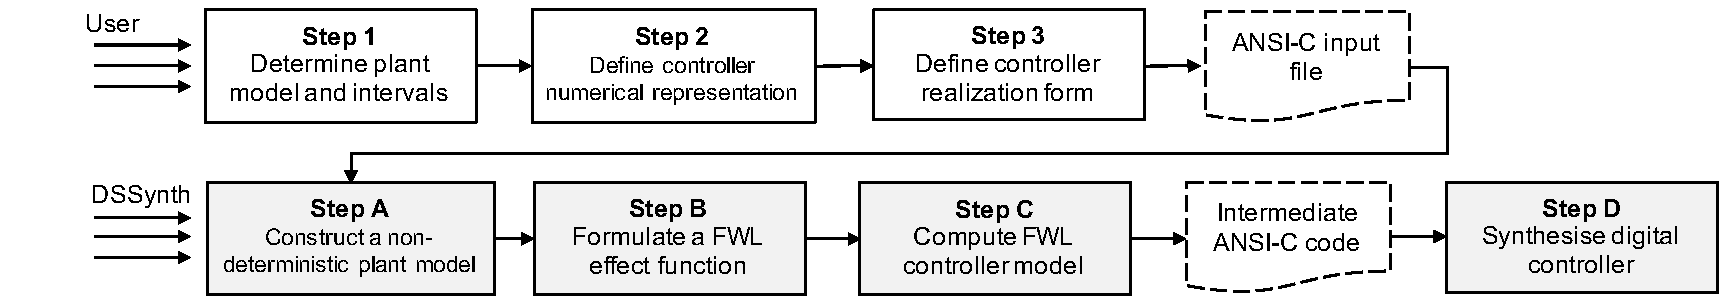
\includegraphics[width=\textwidth]{figures/verification-flow.pdf}
\vspace{1ex}
\caption{Overview of the synthesis process\label{DSSynth_process}}
\end{figure*}

%In Step $1$, the user provides inputs $G(z)$ and $\Delta{G}(z)$
%%$\%$ ({\it i.e.}, $\Delta{G}(z)$ as a percentage of $G(z)$)
%, which contain the plant model and the
%interval, respectively.  In Step $2$, a digital controller must be designed
%with any preferred method, where $C(z)$ is obtained.  The controller
%numerical representation and realization form are chosen in Steps $3$ and
%$4$, respectively.  In Step $5$, the user finally configures the
%verification parameters ({\it e.g.}, verification time, properties, and BMC
%tool).  After that, DSVerifier verification engine performs an (automatic)
%verification of the desired property $\phi$ ({\it i.e.}, stability).  The
%user steps described in Steps $1$--$5$ result in an ANSI-C code that should
%be used as an input for DSVerifier.

Given a model for a plant in ANSI-C syntax as input (Steps 1--3), \tool
constructs a non-deterministic model to represent the plant family (Step~A),
and formulates a function (Step~B) using implementation details provided in
Steps~$2$ and $3$ to calculate the parameters of the controller to be
synthesized (Step~C).  Finally, \tool builds an intermediate ANSI-C code for
the digital system implementation, which is used as input for the CEGIS
engine (Step~D).

This intermediate ANSI-C code model contains a specification $\phi$ for the
property of interest (i.e., robust stability) and is passed to the
Counterexample-Guided Inductive Synthesis (CEGIS) module of
CBMC~\cite{ClarkeKL04}, where the controller is marked as the input variable
to synthesize.  CEGIS employs an iterative, counterexample-guided refinement
process, which is explained in detail in Section~\ref{synthesizer-general}. 
CEGIS reports a successful synthesis result if it generates a controller
that is safe with respect to~$\phi$.  In particular, the ANSI-C code model
guarantees that a synthesized solution is complete and sound with respect to
the stability property~$\phi$, since it does not depend on system inputs and
outputs.  In the case of stability, the specification~$\phi$ consists of a
number of assumptions on the polynomial coefficients, following Jury's
Criteria, as well as the restrictions on the representation of these
coefficients as discussed in detail in Section~\ref{synthesis-elements}.

% by the function $f$ (cf.~Eq.~\eqref{FWL_tf})
%In Step A, DSVerifier constructs a non-deterministic model to represent the
%plant family $\mathfrak{G}$ using $g_0$ and $\Delta{g}\%$, which are
%provided in Step $1$.  DSVerifier then formulates $\mathit{FWL}[\cdot]$ in
%Step B using implementation details provided from Steps $2$ and $3$, and
%then computes $\mathit{FWL}[c_0]$ in Step C.  Thus, DSVerifier builds an
%intermediate ANSI-C code for the digital system implementation, which is
%used as input for the model-checker, as pointed in Step D.

%This intermediate ANSI-C code model has three main modules: digital
%controller code to be embedded into the microprocessor; plant model code,
%which simulates the plant model dynamics considering uncertainties; and
%``assert'' and ``assume'' statements, which control the verification flow. 
%For the digital controller code, transfer functions coefficients are
%quantised and deterministic, and all operations use fixed-point arithmetic. 
%\textcolor{red}{In the plant model code, transfer function coefficients are
%not quantised, but represented with maximum precision based on float
%data-type variables}; they are treated as non-deterministic variables to
%support model uncertainties.  The directive ``assume'' bounds
%non-deterministic variables, {\it i.e.}, inputs and plant uncertain
%coefficients.
%
%The translation of ANSI-C code into SAT/SMT formulae
%is done by a back-end model-checking tool ({\it e.g.},
%CBMC~\cite{ClarkeKL04} or ESBMC~\cite{CordeiroFM12}).  Here, DSVerifier
%symbolically checks a given property $\phi$ with respect to closed-loop
%systems, which are composed by $f(c_i)$ and every $G$ in $\mathfrak{G}$. 
%If any property violation is found, then DSVerifier reports a
%counterexample, which contains system inputs or parametric deviations
%$\Delta{G}$ that lead the system to a failure.  A successful verification
%result is reported if the system is safe with respect to $\phi$.  In
%particular, the stability verification is complete and sound, since it does
%not depend on system outputs and inputs.

%%%%%%%%%%%%%%%%%%%%%%%%%%%%%%%%%%%%%%%%%%%%%%%%%%%%%%%%%%%%%%%%%%%%%%%%%%%%%%%%%%%%%%
%\section{Modelling Errors} 

%In this section, we show how to embed discretization errors on the plant model, as follows: 
%%$\hat{G}(z)$ is split into two terms:
%%
%\begin{equation}
%\label{eq:uncertainplant}
%%\hat{G}(z)=G(z)+\Delta{G(z)},
%\tilde G(z) = \hat G(z) + \Delta G_P(z) = G(z,T) + \Delta G_Q(z) + \Delta G_P(z),   
%\end{equation}
%where $G(z,T)$ is the time discretization of the nominal physical plant $G(s)$, 
%$\Delta{G_{Q}(z)}$ represents the quantization uncertainty model, 
%and $\Delta{G_{P}(z)}$ describes the parametric uncertainty model. 

%\noindent where $G(z)$ is the discretised nominal plant model and
%$\Delta{G(z)}$ is the additive uncertainty, which is related to parametric
%uncertainties~\cite{Bessa16}.  

%\section{An Uncertainty Model for the quantization Error} 
%\label{sec:uncertainty-model-quantization-error}
%
%%Here, an uncertainty model to accommodate the
%%quantization noise effects on $\hat{G}(z)$ is proposed.  
%%As a result, Eq.~\eqref{eq:uncertainplant} is rewritten as
%%
%%\begin{equation}
%%\label{eq:uncertainFWLplant}
%%\hat{G}(z)=G(z)+\Delta{G_{Q}(z)}+\Delta{G_{P}(z)},
%%\end{equation}
%
%A model for $\Delta{G_{Q}(z)}$ that can represent the quantization
%noise effect in the plant output, and consequently the closed-loop system
%output, is proposed.  
%%\red{[eliminate next:] 
%%For convenience, the parametric uncertainties will be described here.}
%
%Consider the closed-loop sampled system in Figure~\ref{fig:sampledsystem},
%where $C(z)$ is the digital controller model, whose control output signal is
%quantised ($Q2$) and interpolated via a ZOH using digital-to-analog
%converter (DAC).  The quantization occurs because the DAC resolution may be
%different from the fixed point representation of the controller.  $G(s)$ is
%the continuous-time model of the plant, from which output samples are taken
%and quantised ($Q1$) by means of an analog-to-digital converter (ADC)
%synchronized with the DAC.  Each quantiser ($Q1$ and $Q2$) will present some
%contribution for the total quantization noise.
%    
%\begin{figure*}[ht]
%\centering
%
%\tikzset{add/.style n args={4}{
%    minimum width=6mm,
%    path picture={
%        \draw[circle] 
%            (path picture bounding box.south east) -- (path picture bounding box.north west)
%            (path picture bounding box.south west) -- (path picture bounding box.north east);
%        \node[draw=none] at ($(path picture bounding box.south)+(0,0.13)$)     {\small #1};
%        \node[draw=none] at ($(path picture bounding box.west)+(0.13,0)$)      {\small #2};
%        \node[draw=none] at ($(path picture bounding box.north)+(0,-0.13)$)    {\small #3};
%        \node[draw=none] at ($(path picture bounding box.east)+(-0.13,0)$)     {\small #4};
%        }
%    }
% }
%
%\resizebox{.8\textwidth}{!}{
% \begin{tikzpicture}[scale=0.6,-,>=stealth',shorten >=.2pt,auto,
%     semithick, initial text=, ampersand replacement=\&,]
%
%  \matrix[nodes={draw, fill=none, shape=rectangle, minimum height=.2cm, minimum width=.2cm, align=center}, row sep=.6cm, column sep=.3cm] {
%    \node[draw=none] (r) {$\tilde R(z)$};
%%   \& \coordinate (aux0);
%   \& \node[circle,add={-}{+}{}{}] (circle) {};
%   \node[draw=none] (ez) at ([xshift=1cm,yshift=.15cm]circle)  {$\tilde e(z)$};
%   \& \node[rectangle,draw,
%	minimum width=1cm,
%	minimum height=1cm,
%        label=\textbf{Controller}] (cz) {{\sc C(z)}};
%   \node[draw=none] (ud) at ([xshift=1cm,yshift=.15cm]cz)  {$\tilde U(z)$};
%     
%   \& complexnode/.pic={ 
%      \node[rectangle,draw,
%	minimum width=3cm,
%	minimum height=1.6cm,
%	label=\textbf{DAC},] (dac) {};
%     \node[circle,add={}{+}{+}{},fill=yellow!20] (q2) at ([xshift=-.65cm]dac.center) {};
%     \node[draw=none] (q2t)  at ([xshift=-.65cm,yshift=-.65cm]dac.center) {{\sc Q2}};
%     \node[draw=none] (v2)  at ([xshift=-.65cm,yshift=1.5cm]dac.center) {$\nu_2(z)$};
%     \node[fill=yellow!20] (zoh) at ([xshift=.65cm]dac.center) {{\sc ZOH}};}
%   \& \node[rectangle,draw,
%	minimum width=1cm,
%	minimum height=1cm,
%        label=\textbf{Plant}] (gs) {{\sc G(s)}};
%   \node[draw=none] (ud) at ([xshift=-1cm,yshift=.15cm]gs)  {$U(s)$};
%   \node[draw=none] (y) at ([xshift=1cm,yshift=.15cm]gs)  {$Y(s)$};
%   \& complexnode/.pic={ 
%     \node[rectangle,draw,
%	minimum width=4cm,
%	minimum height=1.6cm,
%	label=\textbf{ADC},] (adc) {};
%   \draw[] ([xshift=-1cm]adc.center) -- ++(0.5,0.2cm);
%   \coordinate (switch1) at ([xshift=-1cm]adc.center);
%   \coordinate (switch2) at ([xshift=-0.4cm]adc.center);
%   \node[circle,add={}{+}{+}{},fill=yellow!20] (q1) at ([xshift=1cm]adc.center) {};} 
%     \node[draw=none] (q2t)  at ([xshift=1cm,yshift=-.65cm]adc.center) {{\sc Q1}};
%   \node[draw=none] (v1)  at ([xshift=1cm,yshift=1.5cm]adc.center) {$\nu_1(z)$};
%   \& \coordinate (aux1);
%   \& \node[draw=none] (yz) {$\tilde Y(z)$};\\
%   \& \coordinate (aux3); 
%   \&
%   \&
%   \& 
%   \& 
%   \& \coordinate (aux2);\\
%  };
%
%
%  \path[->] (v1) edge (q1.north);
%  \path[->] (v2) edge (q2.north);
%  \path[->] (r) edge (circle.west);
%  \path[->] (aux1) edge (yz);
%  \path  
%   (circle.east) edge (cz)
%   (cz.east) edge (q2.west)
%   (q2.east) edge (zoh.west)
%   (zoh.east) edge (gs.west)
%   (switch2) edge (q1.west)
%   (q1.east) edge (aux1.west)
%   (gs.east) edge (switch1.west)
%   (aux1.south) edge (aux2.north)
%   (aux2.west) edge (aux3.east); 
%  \path[->]  (aux3.north) edge (circle.south);
% \end{tikzpicture}
%}
% \caption{Sampled System. \label{fig:sampledsystem}}
%\end{figure*}
%
%%% \begin{figure}[ht]
%%% \centering
%%% 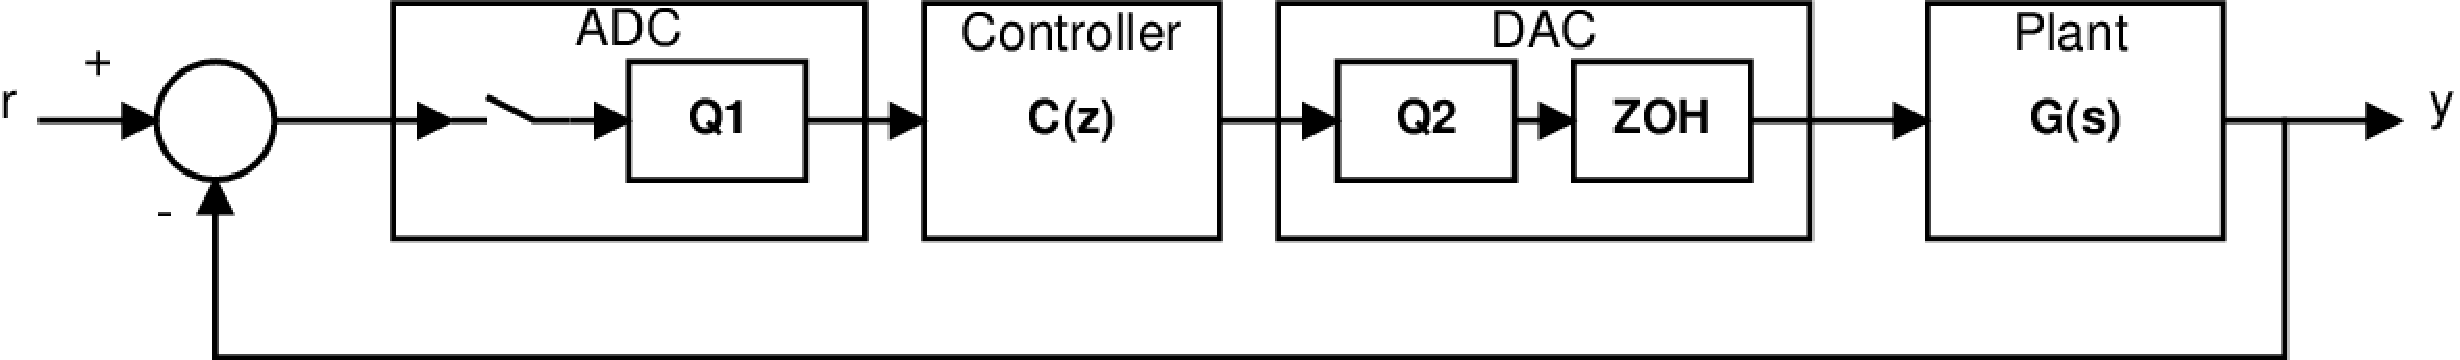
\includegraphics[width=\columnwidth]{figures/hsystembd.pdf}
%%% \caption{Sampled system.}
%%% \label{fig:sampledsystem}
%%% \end{figure}
%
%
%\begin{figure}[ht]
%\centering
%
%\tikzset{add/.style n args={4}{
%    minimum width=6mm,
%    path picture={
%        \draw[circle] 
%            (path picture bounding box.south east) -- (path picture bounding box.north west)
%            (path picture bounding box.south west) -- (path picture bounding box.north east);
%        \node[draw=none] at ($(path picture bounding box.south)+(0,0.13)$)     {\small #1};
%        \node[draw=none] at ($(path picture bounding box.west)+(0.13,0)$)      {\small #2};
%        \node[draw=none] at ($(path picture bounding box.north)+(0,-0.13)$)    {\small #3};
%        \node[draw=none] at ($(path picture bounding box.east)+(-0.13,0)$)     {\small #4};
%        }
%    }
% }
%
%\resizebox{.5\textwidth}{!}{
% \begin{tikzpicture}[scale=0.3,-,>=stealth',shorten >=.2pt,auto,
%     semithick, initial text=, ampersand replacement=\&,]
%
%  \matrix[nodes={draw, fill=none, shape=rectangle, minimum height=.2cm, minimum width=.2cm, align=center}, row sep=.6cm, column sep=.3cm] {
%    \node[draw=none] (r) {$R(z)$};
%%   \& \coordinate (aux0);
%   \& \node[circle,add={-}{+}{}{}] (circle) {};
%   \node[draw=none] (ez) at ([xshift=1cm,yshift=.15cm]circle)  {$e(z)$};
%   \& \node[rectangle,draw,
%	minimum width=1cm,
%	minimum height=1cm,
%        label=\textbf{Controller}] (cz) {{\sc C(z)}};
%   \node[draw=none] (ud) at ([xshift=1cm,yshift=.15cm]cz)  {$U(z)$};
%   \& \node[rectangle,draw,
%	minimum width=1cm,
%	minimum height=1cm,
%        label=\textbf{Plant}] (gs) {{\sc G(z)}};
%   \node[draw=none] (y) at ([xshift=1cm,yshift=.15cm]gs)  {$Y(z)$};
%
%   \& \node[circle,add={}{+}{+}{}] (circle2) {};
%%   \node[draw=none] (tyz) at ([xshift=-1cm,yshift=.15cm]circle2)  {$Y(z)$};
%   \node[draw=none] (nu) at ([yshift=1cm]circle2)  {$\nu(z)$};
%   \& \coordinate (aux1);
%   \& \node[draw=none] (yz) {$\tilde Y(z)$};\\
%   \& \coordinate (aux3); 
%   \&
%   \& 
%   \& 
%   \& \coordinate (aux2);\\
%  };
%
%
%%  \path[->] (v1) edge (q1.north);
%%  \path[->] (v2) edge (q2.north);
%  \path[->] (r) edge (circle.west);
%  \path[->] (nu) edge (circle2.north);
%  \path[->] (aux1) edge (yz);
%  \path  
%   (circle.east) edge (cz)
%   (cz.east) edge (gs.west)
%   (gs.east) edge (circle2.west)
%   (circle2.east) edge (aux1.west)
%   (aux1.south) edge (aux2.north)
%   (aux2.west) edge (aux3.east); 
%  \path[->]  (aux3.north) edge (circle.south);
% \end{tikzpicture}
%}
% \caption{Sampled System. \label{fig:sampledsystem}}
%\end{figure}
%
%%
%%
%
%\begin{figure}[ht]
%\centering
%
%\tikzset{add/.style n args={4}{
%    minimum width=6mm,
%    path picture={
%        \draw[circle] 
%            (path picture bounding box.south east) -- (path picture bounding box.north west)
%            (path picture bounding box.south west) -- (path picture bounding box.north east);
%        \node[draw=none] at ($(path picture bounding box.south)+(0,0.13)$)     {\small #1};
%        \node[draw=none] at ($(path picture bounding box.west)+(0.13,0)$)      {\small #2};
%        \node[draw=none] at ($(path picture bounding box.north)+(0,-0.13)$)    {\small #3};
%        \node[draw=none] at ($(path picture bounding box.east)+(-0.13,0)$)     {\small #4};
%        }
%    }
% }
%
%\resizebox{.5\textwidth}{!}{
% \begin{tikzpicture}[scale=0.3,-,>=stealth',shorten >=.2pt,auto,
%     semithick, initial text=, ampersand replacement=\&,]
%
%  \matrix[nodes={draw, fill=none, shape=rectangle, minimum height=.2cm, minimum width=.2cm, align=center}, row sep=.6cm, column sep=.3cm] {
%    \node[draw=none] (r) {$R(z)$};
%%   \& \coordinate (aux0);
%   \& \node[circle,add={-}{+}{}{}] (circle) {};
%   \node[draw=none] (ez) at ([xshift=1cm,yshift=.15cm]circle)  {$e(z)$};
%   \& \coordinate (aux4);
%   \& \node[rectangle,draw,
%	minimum width=1cm,
%	minimum height=1cm,
%        label=\textbf{Controller}] (cz) {{\sc C(z)}};
%   \node[draw=none] (ud) at ([xshift=1cm,yshift=.15cm]cz)  {$U(z)$};
%   \& \node[rectangle,draw,
%	minimum width=1cm,
%	minimum height=1cm,
%        label=\textbf{Plant}] (gs) {{\sc G(z)}};
%   \node[draw=none] (y) at ([xshift=1cm,yshift=.15cm]gs)  {$Y(z)$};
%   \& \node[circle,add={+}{+}{}{}] (circle2) {};
%%   \node[draw=none] (tyz) at ([xshift=-1cm,yshift=.15cm]circle2)  {$Y(z)$};
%%   \node[draw=none] (nu) at ([yshift=1cm]circle2)  {$\nu(z)$};
%   \& \coordinate (aux1);
%   \& \node[draw=none] (yz) {$\tilde Y(z)$};\\
%   \& 
%   \& \coordinate (aux5); 
%   \& \node[rectangle,draw,
%	minimum width=1cm,
%	minimum height=1cm] (deltag) {{\sc $\Delta G(z)$}};
%   \&
%   \& \coordinate (aux6);\\
%   \& \coordinate (aux3); 
%   \&
%   \& 
%   \& 
%   \&
%   \& \coordinate (aux2);\\
%  };
%
%
%%  \path[->] (v1) edge (q1.north);
%%  \path[->] (v2) edge (q2.north);
%  \path[->] (r) edge (circle.west);
%%  \path[->] (nu) edge (circle2.north);
%  \path[->] (aux1) edge (yz);
%  \path  
%   (aux4.north) edge (aux5.south)
%   (aux5.east) edge (deltag.west)
%   (deltag.east) edge (aux6.west)
%   (aux6.south) edge (circle2.south)
%   (circle.east) edge (cz)
%   (cz.east) edge (gs.west)
%   (gs.east) edge (circle2.west)
%   (circle2.east) edge (aux1.west)
%   (aux1.south) edge (aux2.north)
%   (aux2.west) edge (aux3.east); 
%  \path[->]  (aux3.north) edge (circle.south);
% \end{tikzpicture}
%}
% \caption{Sampled System. \label{fig:sampledsystem}}
%\end{figure}




%\begin{myprop}
%Considering the quantization noise $\nu(k)$ as an output error in the
%discrete plant model, 
%%{\it i.e.}, it does not affect the plant dynamics, but its output samples, 
%$\Delta{G_{Q}(z)}$ can be obtained from
%%
%\begin{equation}
%\label{eq:quantization_tf}
%\Delta{G_{Q}(z)}=\frac{\nu(z)}{U(z)},
%\end{equation}
%where $\nu(z)$ is the z-transform of the random process $\nu(k)$,
%which can be calculated through the power spectral density of
%$\nu(k)$~\cite{poularikas2000transforms}.  
%Thus, the $\Delta{G_{Q}(z)}$ can expressed as
%%
%\begin{equation}
%\label{eq:deltag_var}
%\Delta{G_{Q}(z)}=\frac{\sigma_{Q}^{2}}{U(z)},
%\end{equation}
%where $\sigma_{Q}^{2}$ is the variance of the quantization noise and
%$U(z)$ is the z-transform of control signal ({\it i.e.}, the z-transform of
%the signal from the digital controller), which is provided to the plant by
%means of ZOH.
%\end{myprop}
%
%%
%\begin{proof}
%%
%Suppose that the plant discrete model in Figure~\ref{fig:sampledsystem} can
%be represented by the following pulse transfer function (without
%quantization noise effect):
%%
%\begin{equation}
%\label{eq:tfwithout}
%G(z)=\frac{Y(z)}{U(z)}=\frac{B(z)}{A(z)}=\frac{b_{0}+b_{1}z^{-1}+b_{2}z^{-2}+\cdots+b_{M}z^{-M}}{1+a_{1}z^{-1}+a_{2}z^{-2}+\cdots+a_{N}z^{-N}},
%\end{equation}
%%
%\noindent where $Y(z)$ is the z-transform of the plant output signal without
%noise $y(k)$, $U(z)$ is the z-transform of the control signal, which is
%provided to the plant, $A(z)$ and $B(z)$ are the plant pulse transfer
%function numerator and denominator, respectively.
%
%Considering the quantization noise $\nu(k)$ as an output error in the
%discrete plant model, an additive noise in the plant output $y(k)$ resulting
%in the noisy output $\hat{y}(k)$ can be represented as
%%
%\begin{equation}
%\hat{y}(k)=y(k)+\nu(k).
%\end{equation}
%
%Note that the model in Eq.~\eqref{eq:tfwithout} is equivalent to the
%following difference equation:
%%
%\begin{equation}
%\begin{split}
%y(k)=-a_{1}y(k-1)-a_{2}y(k-2)-\cdots - a_{N}y(k-N)\\
%+b_{0}u(k)+b_{1}u(k-1)+b_{2}u(k-2)+\cdots+b_{M}u(k-M),
%\end{split}
%\end{equation}
%
%\noindent and consequently $\hat{y}(k)$ can be represented by the following
%difference equation:
%%
%\begin{equation}
%\label{eq:differencewithnoise}
%\begin{split}
%\hat{y}(k)=-a_{1}y(k-1)-a_{2}y(k-2)-\cdots - a_{N}y(k-N)\\
%+b_{0}u(k)+b_{1}u(k-1)+b_{2}u(k-2)+\cdots+b_{M}u(k-M)+\nu(k).
%\end{split}
%\end{equation}
%
%The z-transform of Eq.~\eqref{eq:differencewithnoise} is
%%
%\begin{equation}
%\begin{split}
%\hat{Y}(z)=(-a_{1}z^{-1}-a_{2}z^{-2}-\cdots-a_{N}z^{-N})Y(z)\\
%+(b_{0}+b_{1}z^{-1}+b_{2}z^{-2}+\cdots+b_{M}z^{-M})U(z)+\nu(z),
%\end{split}
%\end{equation}
%dividing both sides by $U(z)$, it is equivalent to:
%\begin{equation}
%\frac{\hat{Y}(z)}{U(z)}=\hat{G}(z)=[1-A(z)]G(z)+U(z)B(z)+\frac{\nu(z)}{U(z)}.
%\end{equation}
%
%Considering $\hat{G}(z)=G(z)+\Delta{G_{Q}(z)}$ and Eq.~\eqref{eq:tfwithout},
%the intended expression can be obtained as
%%
%\begin{equation}
%\Delta{G_{Q}(z)}=\frac{\nu(z)}{U(z)} 
%\end{equation}
%\end{proof}

%Eq.~\eqref{eq:deltag_var} indicates that the modelling of the quantization noise
%effect on the plant transfer function demands an estimation of the variance
%of quantization noise $\sigma_{Q}^{2}$.  To obtain such estimation, the
%methodology presented by~\cite{widrow2008quantization}
%is used.  The authors provide an algorithm for computing the mean square of
%the output noise due to $Q1$ and $Q2$.  Considering that each quantiser
%contribution can be represented by a white noise with zero mean
%(Assumption~\ref{whitenoise}), the mean square can be considered as the
%variance of noise ($\sigma_{Q}^{2}$), which can be calculated as
%%
%\begin{equation}
%\sigma_{Q}^{2}=\frac{\lambda_{1}^{2}\cdot \sum {h_{Q1}^{2}} \cdot q_{1}+\lambda_{2}^{2}\cdot \sum {h_{Q2}^{2}} \cdot q_{2}}{12},
%\end{equation}
%%
%\noindent where $\lambda_{1}$ and $\lambda_{2}$ are the scale factors, {\it i.e.} constant gains usually employed before the ADC and after the DAC in order to avoid the overload of converters  %\red{[define scale factors]} 
%for the quantization $Q1$ and $Q2$, respectively; $q_{1}$ and $q_{2}$ are the quantization step for $Q1$ and $Q2$, respectively, and $\sum {h_{Q1}^{2}}$ and $\sum
%{h_{Q2}^{2}}$ are the squares sums of the impulse response obtained by means
%of a transfer function from $Q1$ and $Q2$ to the plant output, respectively.
%
%The transfer functions $H_{Q1}(z)$ and $H_{Q2}(z)$, from which the squares
%sums of the impulse response are needed, can be obtained through the
%analysis of the system in Figure~\ref{fig:sampledsystem}. 

%\red{[The following text needs to be completed. (Notice typos, reference to wrong signal $R$, and to wrong TF $C,G$.]}
%
%Considering that
%the quantiser $Q1$ is the source of a white noise with zero mean $\nu_{1}$
%and $Q2$ is the source of a white noise with zero mean $\nu_{2}$, the
%following equation can be written for the system in
%Figure~\ref{fig:sampledsystem}
%%
%\begin{equation}
%\resizebox{0.48\textwidth}{!}{
%$\tilde{Y}(z)=\tilde R(z)C(z)G(z)-\tilde{Y}(z)C(z)G(z)+\nu_{1}(z)+\nu_{2}(z)G(z),$
%}
%\end{equation}
%
%\noindent which can be rewritten as
%%
%\begin{equation}
%\label{eq:outputfunctions}
%\tilde{Y}(z)=C(z)G(z)H(z)R(z)+H(z)\nu_{1}(z)+G(z)H(z)\nu_{2}(z)
%\end{equation}
%$$H(z)=\frac{1}{1+C(z)G(z)}$$
%
%Note that $H(z)$ cancels the poles of both $G(z)$ and $C(z)$, thus we need only verify the stability of $H(z)$
%to validate the stability of the whole system.
%These equations are sufficient for computing $\sigma_{Q}^{2}$.  However,
%there is still a gap for a complete model for $\Delta{G_{Q}(z)}$ in
%Eq.~\eqref{eq:deltag_var}, {\it i.e.}, the z-transform of control action
%$U(z)$.  This indicates that the quantization noise effect on a discrete
%plant model mainly depends on three main factors:
%%
%\begin{itemize}
%%
%\item \textbf{Sample time:} the sample time effect is reflected over pulse transfer function that covers the effects of DAC ant its interpolator (ZOH) \red{[clarify/revise based on the comments made above.]};
%%
%\item \textbf{ADC and DAC step:} \red{[again, do we need both?]} these are the main component of quantization noise power, but an $8$-bits converter already reduces the effect of quantization noises in the output for negligible values.
%%
%\item \textbf{Signal-to-noise ratio (SNR): } the dependence on the value of $U(z)$ \red{[notice that now we have reduced the problem to depend on the effect of the reference signal transform R(z) - pls revise.]} shows the importance of the SNR for handling quantization noise; for a high SNR of the digital controller, the quantization effect is negligible. This happens during the transient of the system, when high control actions are employed. However, it can be relevant during the steady state. A digital controller with integral action might be sufficient for eliminating such influence at steady state.
%%
%\end{itemize}
%
%An alternative expression for $\Delta{G_{Q}(z)}$ can be obtained from
%Eq.~\eqref{eq:deltag_var}, transforming it into a function of the reference
%$R(z)$.  Once $U(z)$ is the control signal obtained via digital controller
%$C(z)$ and error signal, {\it i.e.},
%%
%\begin{equation}
%U(z)=C(z)\cdot[R(z)-Y(z)],
%\end{equation} 
%
%\noindent where $Y(z)$ is the first term of Eq.~\eqref{eq:outputfunctions}, thus:
%\begin{equation}
%\label{eq:controlsignal}
%\resizebox{0.48\textwidth}{!}{
%$U(z)=C(z)\cdot \left[R(z)-\frac{C(z)G(z)}{1+C(z)G(z)}R(z)\right]=\frac{C(z)}{1+C(z)G(z)}R(z).$
%}
%\end{equation} 
%
%Substituting Eq.~\eqref{eq:controlsignal} in Eq.~\eqref{eq:deltag_var}, a
%model for $\Delta{G_{Q}(z)}$ depending on $R(z)$ can be obtained:
%%
%\begin{equation}
%\Delta{G_{Q}(z)}=\sigma^{2}_{Q}\cdot \frac{1+C(z)G(z)}{C(z)} \cdot \frac{1}{R(z)},
%\end{equation}
%
%\noindent where $R(z)$ can be considered as a step signal (for stabilization
%purpose) with height equal to $r$, which can be rewritten as
%%
%\begin{equation}
%\Delta{G_{Q}(z)}=\frac{\sigma^{2}_{Q}}{r}\cdot \frac{1+C(z)G(z)}{C(z)} \cdot \frac{z-1}{z}.
%\end{equation}
%
%A more precise description of $\Delta{G_{Q}(z)}$ can be obtained
%considering FWL \red{[clarify what you mean with FWL, introduce FWL function explicitly and precisely]} effects on digital controller coefficients, as described in
%Bessa {\it et al.}~\cite{Bessa16}, {\it i.e.}, using $FWL[C(z)]$ instead of
%the nominal $C(z)$:
%%
%\begin{equation}
%\label{eq:deltaG_final}
%\Delta{G_{Q}(z)}=\frac{\sigma^{2}_{Q}}{r}\cdot \frac{1+FWL[C(z)]G(z)}{FWL[C(z)]} \cdot \frac{z-1}{z}.
%\end{equation}
%
%Finally, Eq.~\eqref{eq:deltaG_final} is a suitable frequency domain model
%for quantization noise effects on closed-loop systems.  This model depends
%on the plant pulse transfer function ($G(z)$), which is described by
%Eq.~\eqref{eq:pulsetf}, the height of step reference signal $r$, and the
%digital controller model.

%\subsection{Modelling Error on Parameters Representation} 
%\label{sec:}

%\red{[TO BE COMPLETED.]}
% We use CounterExample-Guided Inductive Synthesis (CEGIS), as
% illustrated in Fig~\ref{fig:CEGIS}.

%specialised it for stream refactoring.  
% adding JST for stream refactoring

\subsection{Architecture of the program synthesizer}
\label{synthesizer-general}
%
%% \red{[I would recommend to clarify the domain of definition of $\sigma$, particularly over the set where $x$ ranges over. 
%% (Be cognisant that control audience might be unfamiliar with the cegis architecture.) ]}
% 
The input specification provided to the program synthesizer is of the form
$\exists \vec{P} .  \forall \vec{x}.  \sigma(\vec{x}, \vec{P})$ where
$\vec{P}$ ranges over functions, $\vec{x}$ ranges over ground terms and
$\sigma$ is a quantifier-free formula.  We interpret the ground terms over
some finite domain $\mathcal{D}$.

The design of our synthesizer is given in Figure~\ref{fig:CEGIS} and consists
of two phases, {\sc Synthesize} and {\sc Verify}, which interact via a
finite set of test vectors {\sc inputs} that is updated incrementally. 
Given the aforementioned specification $\sigma$, the {\sc synth} procedure
tries to find an existential witness $\vec{P}$ satisfying the specification
$\sigma(\vec{x}, \vec{P})$ for all $\vec{x}$ in {\sc inputs} (as opposed to
all $\vec{x} \in \mathcal{D}$).
%
If {\sc synthesize} succeeds in finding a witness~$\vec{P}$, this witness
is a candidate solution to the full synthesis formula.  We pass this
candidate solution to {\sc verify}, which checks whether it is a full
solution (i.e., $\vec{P}$ satisfies the specification $\sigma(\vec{x},
\vec{P})$ for all $\vec{x}\in\mathcal{D}$).
%
%determines whether
%it does satisfy the specification on all inputs by checking
%satisfiability of the following verification formula:
%
%$\exists \vec{x} . \lnot \sigma(\vec{x}, \vec{P})$
%If this formula is unsatisfiable, 
%% the candidate solution is in fact a 
%% full solution.
%
If this is the case, then the algorithm terminates.  Otherwise, additional
information is provided to the {\sc synthesize} phase in the form of a new
counterexample that is added to the {\sc inputs} set and the loop iterates
again (note that, for now, we ignore the second feedback signal ``Increase
Precision'' provided by the {\sc Verify} phase in Figure~\ref{fig:CEGIS} as it
is specific to control synthesis and will be described in the next section).

%% the witness $\vec{x}$ denote an input on which the
%% candidate solution fails to meet the specification.  Thus, $\vec{x}$ is
%% added to the {\sc inputs} set, and the loop iterates again.  

It is
worth noting that each iteration of the loop adds a new input to the
finite set $\text{\sc inputs}$ that is used for synthesis.  Given that
the full set of inputs $\mathcal{D}$
%\blue{[which by now should have a name, as suggested to be introduced above]} 
is finite, this means that the refinement loop
can only iterate a finite number of times.

\subsection{Synthesis for control}
\label{synthesis-elements}

\paragraph{Specification of the stability property}

Next, we describe the specific property that we pass to the program
synthesizer as the specification $\sigma$.  There are two different
algorithms in DSVerifier that can be used for stability
verification~\cite{daes20161, Bessa16}, one based on Schur's decomposition
and another one based on Jury's criteria~\cite{astrom1997computer}.  Here,
we choose Jury's method~\cite{astrom1997computer}, due to its efficiency,
and we use this method to check the stability in the $z$-domain for the
characteristic polynomial $S(z)$ defined in~\eqref{eq:internal_stab_lemma}.
%
% of the matrix $\left( \begin{array}{c} Y \\ U \end{array}\right)$, where $Y(z)$ is the closed-loop system output and U(z) is the controller output. 
%% \red{[unclear: what matrix? We need to clarify the relationship
%% between the char. poly. $S(z)$ and the later quantities $\Delta
%% N_{G}(z), \Delta D_{G}(z)$ and corresponding controller's
%% structure.]}.
%
We~consider the following form for $S(z)$:
%
$$
S(z) = a_0z^N+a_1z^{N-1}+\cdots+a_{N-1}z+a_N=0, a_0\neq0
$$
%
%\cdsay{is this for the matrix $\left( \begin{array}{c} Y \\ U \end{array}\right)$?}

% Assuming that $\hat{G}(z) = \frac{\hat{N_G}(z)}{\hat{D_G}(z)}$
% and $\hat{C}(z) = \frac{\hat{N_C}(z)}{\hat{D_C}(z)}$, then:
% $$S(z) = FWL[N_C(z)] \times \hat{N_G}(z) + FWL[D_C(z)] \times \hat{D_G}(z)$$

Next, the following Jury matrix
$M = [m_{ij}]_{(2N-2)\times N}$ is built from $S(z)$ coefficients:
%
$$
M=\left( 
\begin{array}{c}
V^{(0)}\\
V^{(1)}\\
\vdots\\
V^{(N-2)}
\end{array}
\right), 
$$
%
where $V^{(k)} = [v^{(k)}_{ij} ]_{2\times N}$ such that:
%
$$
v_{ij}^{(0)}=\left\{
\begin{array}{ll}
a_{j-1}, & \texttt{if}~i=1\\
v_{(1)(N-j+1)}^{0},&\texttt{if}~i=2
\end{array}
\right.
$$
%
$$
v_{ij}^{(k)}=\left\{
\begin{array}{ll}
0,&\texttt{if}~j>n-k\\
v_{1j}^{(k-1)}-v_{2j}^{(k-1)} . \frac{v_{11}^{(k-1)}}{v_{21}^{(k-1)}}, & \texttt{if}~j\leq n-k ~\texttt{and}~i=1\\
v_{(1)(N-j+1)}^{k},& \texttt{if}~j\leq n-k ~\texttt{and}~i=2\\
\end{array}
\right.
$$
%
where $k \in \mathbb{Z}$, such that $0 < k < N - 2$. 
$S(z)$ is the
characteristic polynomial of a stable system if and only if the following four conditions hold:
%\begin{itemize}
%\item 
$R_1: S(1) > 0$;
%\item 
$R_2: (−1)^N S(−1) > 0$;
%\item 
$R_3: |a_0| < a_N$;
%\item 
$R_4: m_{11} > 0 \wedge m_{31}>0 \wedge m_{51}>0 \wedge \cdots \wedge m_{(2N{-}3)(1)}>0$.
%\end{itemize}

The stability property is then encoded by creating a
constraint of the form:
$
\phi_\mathit{stability} \equiv (R_1 \wedge R_2 \wedge R_3 \wedge R_4).
$
%\cdsay{figure out what is existentially quantified for the final $\sigma$.} 
%% \red{[Yes, intuitively all clear, however for the sake of clarity I would like to see the explicit mapping between the above formula and the previously used specification 
%% $\sigma(x, P)$, with clear elucidation of the relationship between the domain of $z$ and that of $x$.]}

% \red{[clear elucidation of the mapping between this and the domains used 
% in the general description of the synthesiser]}

\paragraph{Fixed-point computation in program synthesis}

The program synthesis engine uses fixed-point arithmetic.  Specifically, we
use the domain $\mathbb{R}\param{I}{F}$ for the controller's coefficients
and the domain $\mathbb{R}\param{I_p}{F_p}$ for the plant's coefficients,
where $I$ and $F$, as well as $I_p$ and $F_p$, denote the number of bits for
the integer and fractional parts, respectively, and $\mathbb{R}\langle
I_p,F_p \rangle \supseteq \mathbb{R}\langle I,F \rangle$.
%
%the coefficients for $C(z)$ 
%$N_c$ and $D_c$ 
%in the domain $\mathbb{R}\param{I}{F}$, 
%and $\mathbb{R}^{m_C}\param{I}{F}$, respectively, 
%where $n_C$ and $m_C$ denote the order of the corresponding polynomials
%where $I$ and $F$ denote the integer and fractional size, respectively.
%Regarding the plant, its coefficients are this is synthesised over the 
%domain $\mathbb{R}^{n_G+m_G}\param{I_p}{F_p}$, where $n_G$ and $m_G$ 
%denote the order of the polynomials representing the 
%numerator and denominator of the plant's transfer function, respectively. 
%Again, $I_p$ and $F_p$ denote the integer and fractional size, respectively, with
%$\mathbb{R}\langle I_p,F_p \rangle \supseteq \mathbb{R}\langle I,F \rangle$.

Given the use of fixed-point arithmetic, 
we need to examine the effect of discretization during these operations.
Let $\tilde C(z)$ and $\tilde G(z)$ be the transfer functions represented
using fixed-point bit vectors.%  with integer size $I_p$ and fractional
% size $F_p$, whose domain is $\mathbb{R}\langle I_p,F_p \rangle \supseteq \mathbb{R}\langle I,F \rangle$.
%
\begin{align}
\small
\label{digital_controller_plant_tf}
\tilde C(z)&=\frac{\tilde \beta_{0}+\tilde \beta_{1}z^{-1}+...+\tilde \beta_{M_C}z^{-M_C}}{\tilde \alpha_{0}+\tilde \alpha_{1}z^{-1}+...+\tilde \alpha_{N_C}z^{-N_C}}, \\
%\label{plant_tf}
\tilde G(z)&=\frac{\tilde b_{0}+\tilde b_{1}z^{-1}+...+\tilde b_{M_G}z^{-M_G}}{\tilde a_{0}+\tilde a_{1}z^{-1}+...+\tilde a_{N_G}z^{-N_G}}.
\end{align}
 
Since the controller is synthesized in the $\mathbb{R}\langle I,F \rangle$
domain,
%
$$\forall i \leq N_C, j \leq M_C\ \  \tilde \beta_{i} \equiv \beta_{i} \wedge \tilde \alpha_{j} \equiv \alpha_{j} \Leftrightarrow \tilde C(z) \equiv C(z)$$
%
However, given a real plant $\hat{G}(z)$, and a discretizing function
%
\begin{align}
\small
\label{FWL_tf}
&f^p : \mathbb{R} \rightarrow  \mathbb{R}\langle I_p,F_p \rangle \triangleq \tilde x = f^p(x) : \tilde x=x-(x\bmod\tilde x)\\
&\mathit{FWL}_n^p[P \in \mathcal{P}] = \tilde P \in \mathcal{P}^{n}\langle I_p,F_p \rangle : c_i \in \vec{P} \wedge \tilde c_i \in \vec{\tilde{P}}=f^p(c_i)  \nonumber
\end{align}
%
we calculate $\tilde G(z)=\mathit{FWL}_{M_G,N_G}^p(\hat{G}(z))$
%
\begin{align}
% \label{digital_controller_tf}
% \tilde C(z)&=\frac{(\hat{\beta}_{0}+\Delta_q \hat{\beta}_{0}) +...+(\hat{\beta}_{M_C}+\Delta_b \hat{\beta}_{M_C})z^{-M_C}}{(\hat{\alpha}_{0}+\Delta_q \hat{\alpha}_{0})+...+(\hat{\alpha}_{N_C}+\Delta_q \hat{\alpha}_{N_C})z^{-N_G}} \nonumber \\
% &= C(z) =\hat{C}(z) + \Delta{C}_b(z)\\
%
\label{digital_plant_tf}
\tilde G(z)&=\frac{(\hat{b}_{0}+\Delta_b \hat{b}_{0}) +...+(\hat{b}_{M_G}+\Delta_b \hat{b}_{M_G})z^{-M_G}}{(\hat{a}_{0}+\Delta_b \hat{a}_{0})+...+(\hat{a}_{N_G}+\Delta_b \hat{a}_{N_G})z^{-N_G}} \nonumber \\
&\Rightarrow \vec{\tilde G} =\vec{\hat{G}}+\Delta_b{\vec{G}}=\vec{G}+\Delta_p{\vec{G}}+\Delta_b{\vec{G}}.
\end{align}
%
where $\Delta_b\hat{c}_i=\hat{c}_i\bmod \tilde{c}_i$
and $\Delta_b{G}$ represents the plant uncertainty caused by
the rounding off effect.  We may encompass all the uncertainty as
$\Delta{\vec{G}}=\Delta_p{\vec{G}}+\Delta_b{\vec{G}}$. 
Since the complexity of SAT solvers is worst-case exponential in the size of
the problem instance, our algorithm tries to solve the problem first for a
low $I_p$, $F_p$, iteratively increasing the precision if it is insufficient.

\paragraph{Our synthesis problem}
The synthesis problem we are trying to solve is the following:
find a digital controller $C(z)$ %denoted by  $N_c$ and $D_c$ 
that makes the closed-loop system stable 
for all possible uncertainties 
%$\Delta{\vec{p}}$ (\ref{eq:uncertainty}).
$\tilde G(z)$ (\ref{digital_plant_tf}).
%, where we precisely describe 
%$(\Delta N_G, \Delta D_G)$. 
% Note that, similar to the rest of the paper, we use the notation 
% $\tilda{N_G}(z) = N_G(z) + \Delta N_G(z)$ and 
% $\hat{N_C}(z) = N_C(z) + \Delta N_C(z)$.
When mapping back to the notation used for describing the general architecture 
of the program synthesizer, the controller $C(z)$ denotes $P$ and 
$\tilde G(z)$ represents $x$. 

As mentioned above, we compute the coefficients for $C(z)$ 
%$N_c$ and $D_c$ 
in the domain $\mathbb{R}\param{I}{F}$, 
%and $\mathbb{R}^{m_C}\param{I}{F}$, respectively, 
%where $n_C$ and $m_C$ denote the order of the corresponding polynomials
and those for $\tilde G(z)$ in the domain
$\mathbb{R}\langle I_p,F_p \rangle$.
While the controller's precision $\param{I}{F}$ is given, 
we can vary $\param{I_p}{F_p}$ such that 
$\mathbb{R}\langle I_p,F_p \rangle \supseteq \mathbb{R}\langle I,F \rangle$.

\subsection{The {\sc Synthesize} and {\sc Verify} phases}

The {\sc synthesize} phase uses BMC to 
compute a solution $C(z)$. % An important remark is that this 
% controller is synthesised in the $\mathbb{R}\langle I,F \rangle$
% domain.

There are two approaches for the {\sc verify} phase.
% based on the described model.  
The first approach uses interval arithmetic \cite{moore1966interval}
to represent the coefficients
$[{c}_i-\Delta_p{c}_i-\Delta_b{c}_i\ ,\
{c}_i+\Delta_p{c}_i-\Delta_b{c}_i+(2^{-F_p})]$ 
and rounds operations outwards during calculations.  This effectively allows
us to simultaneously evaluate the whole collection of plants $\mathfrak{G}$
plus the effects of numeric calculations in the engine.  Synthesized
controllers using this verifier will always be stable for all plants in the
family.
% and only generate counterexamples when the precision of the
%engine is insufficient (\emph{ie} no stable plant could be found). 
Our preliminary experiments showed that a synthesis approach
using this verification engine has poor performance and we
%Given the high computational cost of this
%approach, 
therefore designed a second approach, which we describe below.
Our experimental results described in Section~\ref{sec:experiments}
%try both approaches and provide the time for the fastest. 
show that the speedup yielded by the second approach 
is in most cases of at least two orders of magnitude.

The second approach is illustrated in Figure~\ref{fig:CEGIS} and uses a
two-stage verification: the first stage performs potentially unsound
fixed-point operations assuming a plant precision \param{I_p}{F_p}, and the
second stage restores soundness by validating these operations using
interval arithmetic on the synthesized controller.
%
\begin{figure*}[htb]
\centering
%\resizebox{1\textwidth}{!}
{
 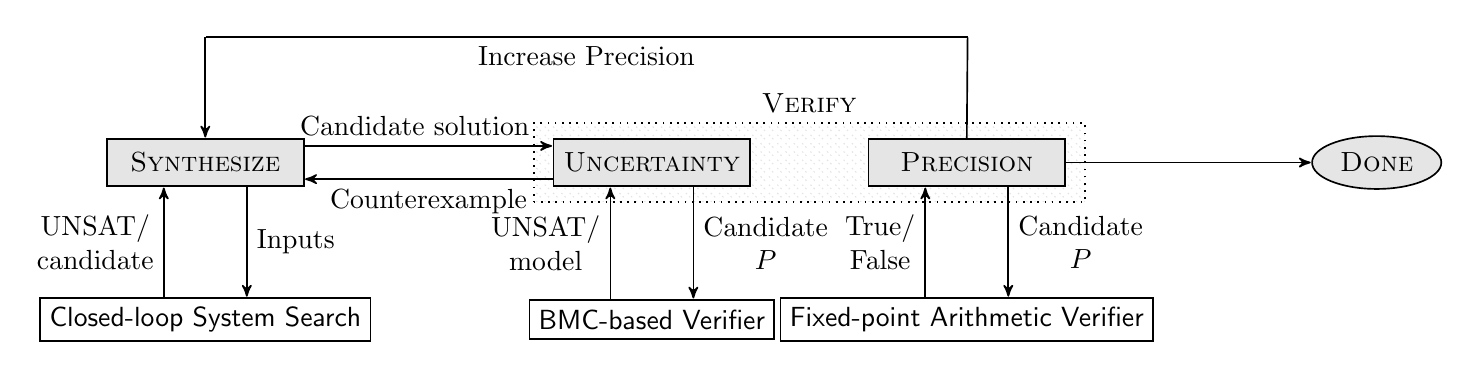
\begin{tikzpicture}[scale=0.3,->,>=stealth',shorten >=.2pt,auto, semithick, initial text=, ampersand replacement=\&,]
  \matrix[nodes={draw, fill=none, shape=rectangle, minimum height=.2cm, minimum width=.2cm, align=center
},
          row sep=.6cm, column sep=2cm] {
   \coordinate (aux1);
   \& \coordinate (aux2);
   \&;\\
   \node[minimum width=2.5cm, minimum height=0.6cm, fill=gray!20] (synth) {{\sc Synthesize}};
   \&
   complexnode/.pic={ 
     \node[rectangle,draw,dotted,
	minimum width=7cm,
	minimum height=1cm,
        pattern=north west lines, pattern color=gray!20,
	label={\sc Verify},] (verif) {};
     \node[minimum width=2.5cm, minimum height=0.6cm, fill=gray!20] (verif1) at ([xshift=-2cm]verif.center) {{\sc Uncertainty}};
     \node[minimum width=2.5cm, minimum height=0.6cm, fill=gray!20] (verif2) at ([xshift=2cm]verif.center) {{\sc Precision}};
   } 
   \& \node[ellipse, fill=gray!20] (done) {{\sc Done}};\\
   %% \node[fill=yellow!20] (verif) {{\sc ~~~~~~Uncertainty~~~~~~}};
   %% \&
   %% \node[fill=yellow!20] (verif2) {{\sc ~~~~~~Precision~~~~~~~}};\\
   \& \\
   \node[minimum height=0.5cm] (gp) {\sf Closed-loop System Search};
   \&
   complexnode/.pic={ 
     \coordinate (aux);
   \node[minimum height=0.5cm] (bmc) at ([xshift=-2cm]aux.center) {\sf BMC-based Verifier};
   \node[minimum height=0.5cm] (fp)  at ([xshift=2cm]aux.center) {\sf Fixed-point Arithmetic Verifier};
   }   
    \\
  };

   \path
    ([yshift=2em]synth.east) edge node[xshift=-0.5em] {Candidate solution} ([yshift=2em]verif1.west)
    ([yshift=-2em]verif1.west) edge node {Counterexample} ([yshift=-2em]synth.east)
    ([xshift=5em]verif1.south) edge node[align=center] {Candidate\\ $P$} ([xshift=5em]bmc.north)
    ([xshift=5em]verif2.south) edge node[align=center] {Candidate\\ $P$} ([xshift=5em]fp.north)
    ([xshift=-5em]bmc.north) edge node[align=center]  {UNSAT/\\model} ([xshift=-5em]verif1.south)
    ([xshift=-5em]fp.north) edge node[align=center]  {True/\\False} ([xshift=-5em]verif2.south)
    (verif2) edge node {} (done)
    ([xshift=5em]synth.south) edge node[align=center] {Inputs} ([xshift=5em]gp.north)
    ([xshift=-5em]gp.north) edge node[align=center] {UNSAT/\\candidate} ([xshift=-5em]synth.south)
    (aux1) edge (synth.north);
   \path[-]
   (verif2.north) edge node[align=center] {} ([xshift=6.7cm]aux2)
   ([xshift=6.7cm]aux2) edge node[align=center] {Increase Precision} (aux1);

 \end{tikzpicture}
}
\caption{Counterexample-Guided Inductive Synthesis of Closed-loop Systems (Step~D)
\label{fig:CEGIS}}
\end{figure*}
%
%
In more detail, in the first stage, denoted by {\sc Uncertainty} in
Figure~\ref{fig:CEGIS}, assuming a precision \param{I_p}{F_p} we check
whether the system is unstable for the current candidate solution, i.e., if
$\neg \phi_\mathit{stability}$ is satisfiable for $S(z)$.  If this is the
case, then we obtain a counterexample $\tilde G(z)$,
%
%denoted by values for each coefficients of $\Delta N_{G}(z)$ and $\Delta D_{G}(z)$, 
%\red{[see my comment above - these quantities pop up too abruptly.]},
%
which makes the closed-loop system unstable.  This uncertainty is added to
the set {\sc inputs} such that, in the subsequent {\sc synthesize} phase, we
obtain a candidate solution consisting of a controller $C(z)$, which makes
the closed-loop system stable for all the uncertainties accumulated in {\sc
inputs}.

If the {\sc Uncertainty} verification stage concludes that the system is
stable for the current candidate solution, then we pass this solution to the
second verification stage, {\sc Precision}, which checks the propagation of
the error in the fixed-point calculations using a Fixed-point Arithmetic
Verifier based on interval arithmetic.
%
% To achieve this, we use a nondeterministic plant selected from $\mathfrak{G}(z)$ where the expected error of the bit vector calculations is assumed to be within the expected bounds and verified after synthesis using the interval version of the program. 
%
% The first verification phase produces a counterexample if some instance of $\mathfrak{G}(z)$ does not verify the properties and the CEGIS loop iteratively looks for a new controller that verifies the supplied counterexamples. The second phase verifies the propagation of the error in the fixed point calculations.
% If the second phase fails verification, we increase the precision of the analyser and feed the CEGIS loop again to find a sound solution. 
% vouches for the use of CEGIS in most of our benchmarks.
% \cdsay{end of integration}

If the {\sc precision} verification returns $\mathit{false}$, then we
increase the precision of \param{I_p}{F_p} and re-start the {\sc
  synthesize} phase with an empty {\sc inputs} set.  Otherwise, we
found a full sound solution for our synthesis problem and we are done.

In the rest of the paper, we will refer to the two approaches 
for the {\sc verify} phase as one-stage and two-stage, respectively.

%%%%%%%%%%%%%%%%%%%%%%%%%%%%%%%%%%%%%%%%%%%%%%%%%%%%%%%%%%%%%%%%%%%%%%%%%%%%%%%%%%%%%%
\subsection{Illustrative Example} \label{sec:running-ex}

We illustrate our approach with a classical cruise control example,
extracted from the literature~\cite{Astrom08}.  The example highlights the
challenges that arise when using finite-precision arithmetic in digital
control.  We are given a discrete plant model (with a time step of
$0.2$\,s), which is represented by the following $z$-expression:
%
\begin{equation}
\label{Eq:running-example-plant}
G(z) = \frac{0.0264}{z-0.9998}.
\end{equation}

Using an optimization tool, the authors
of~\cite{DBLP:conf/hybrid/WangGRJF16} have designed a high-performance
controller for this plant, which is characterized by the following
$z$-domain transfer function:
%
\begin{equation}
\label{Eq:running-example-controller}
C(z) = \frac{2.72z^2 - 4.153z + 1.896}{z^2 - 1.844z + 0.8496}.
\end{equation}
%
The authors of~\cite{DBLP:conf/hybrid/WangGRJF16} claim that this controller
$C(z)$ (Eq.~\eqref{Eq:running-example-controller}) stabilizes the
closed-loop system for the discrete plant model $G(z)$
(Eq.~\ref{Eq:running-example-plant}).  However, if the effects of
finite-precision arithmetic are considered during verification (e.g.,
fixed-point arithmetic and word-length), then this closed-loop system
becomes unstable.
%
For instance, an implementation of $C(z)$ using \param{4}{16} fixed-point
numbers (i.e., $4$ bits for the integer part and $16$ bits for the
fractional part) can be modeled as follows:
%
\begin{equation}
\label{Eq:running-example-controller-quantized}
\resizebox{.47\textwidth}{!}{
$C_{q}(z) {:=} \frac{2.7199859619140625z^2{-}4.1529998779296875z
{+}1.89599609375}{z^2{-}1.843994140625z+0.8495941162109375}$
}
\end{equation} 
%
The resulting system using the typical series loop configuration, where
$C_{q}(z)$ and $G(z)$ are in the forward path, is unstable. 
Figure~\ref{fig:original} gives the Bode diagram for the digital controller
represented by Eq.~\eqref{Eq:running-example-controller}.  The phase margin
is negative, which means that the controller represented by
Eq.~\eqref{Eq:running-example-controller} is unstable, considering FWL
effects.

\subsection{Program synthesis for the example}
%
We now demonstrate how our approach solves the synthesis problem for the
example given in the previous section.  We start with the candidate solution
with all coefficients zero, as given below, and a precision of $I_p=16$,
$F_p=24$.  The digital controller is designed with standard techniques for
control systems~\cite{Kuo:2002:ACS:579453, Ogata:1987:DCS:26170}.
%
%\red{[Be more explicit, write out spurious candidate solution with zero coefficients. KISS - you don't want to lose the control audience here.]}.
%
%$$
%\begin{array}{ll}
%N_C(z) {=} 0z^2{+}0z{+}0\\
%D_C(z) {=} 0z^2{+}0z{+}0\\
%\end{array}
%$$
$$ C(z)=\frac{0z^2{+}0z{+}0}{0z^2{+}0z{+}0} $$

In the first {\sc verify} stage, the {\sc uncertainty} 
check finds the following counterexample:
%
$$ \tilde G(z) = \frac{0.026506}{1.000610z+1.002838} $$

%$$
%\begin{array}{ll}
%\Delta N_G(z) = 0.026506\\
%\Delta D_G(z) = 1.000610z+1.002838
%\end{array}
%$$

We add this counterexample to {\sc inputs} and initiate the {\sc synthesize}
phase, where we obtain the following candidate solution:
%
%\red{[ How is the order of the candidate solution chosen here?]}
$$
C(z)=\frac{12.402664z^2{-}11.439667z{+}0.596756}{4.003906z^2{-}0.287949z{+}0.015625}
$$

This time, the {\sc uncertainty} check does not find any
counterexample and we pass the current candidate solution to the {\sc
precision} verification stage.
%
% In the second {\sc verify} phase, we check whether the current candidate
% solution above is the final solution. It is not and the verifier signals
% that it is due to lack of precision.
%
We obtain the result $\mathit{false}$, meaning that the current precision is
insufficient.  Consequently, we increase our precision to $I_p=20$, $F_p=28$.
%
Since the previous counterexamples were obtained at lower precision, we
remove them from the set of counterexamples.  Back in the {\sc synthesize}
phase, we re-start the process with a candidate solution with all
coefficients $0$.  Next, the {\sc uncertainty} verification stage provides
the first counterexample at higher precision:
%
%$$
%\begin{array}{ll}
%\Delta N_G(z) {=} 0.026314\\
%\Delta D_G(z) {=} 0.999024z{-}1.004785
%\end{array}
%$$
$$ \tilde G(z) = \frac{0.026314}{0.999024z{-}1.004785} $$

In the next {\sc synthesize} phase, we get a new candidate solution that
eliminates the new, higher precision counterexample:
%
$$ C(z)=\frac{11.035202z^2{+}5.846100z{+}4.901855}{1.097901z^2{+}0.063110z{+}0.128357} $$
%
%$$
%\begin{array}{ll}
%N_C(z) {=} \\
%D_C(z) {=} \\
%\end{array}
%$$

This candidate solution is validated as the final solution by both stages
{\sc uncertainty} and {\sc precision} in the {\sc verify} phase. 
Figure~\ref{fig:bode} compares the Bode diagram of the illustrative example
using the digital controller represented by
Eq.~\eqref{Eq:running-example-controller}
from~\cite{DBLP:conf/hybrid/WangGRJF16} (Figure~\ref{fig:original}) and the
final candidate solution from our synthesizer
(Figure~\ref{fig:cegiscontroller}).  The final solution from \tool is stable
since it presents an infinite phase margin and a gain margin of $17.8$\,dB.

%, which fails to find a new counterexample (i.e. returns UNSAT).

% \blue{
% For the same cruise control system, the synthesis may be done considering that the plant model have parametric uncertainties ($\Delta G_{P}(z)$). Thus, the synthesised controller must to stabilize for any parametric variation $\Delta p$ inside of a given region. Specially, in this example, was assumed that each coefficient of $G(z)$ may vary $\pm 0.5\%$.
% }

% \blue{Initially, the controller denominator and numerator  ($D_{C}(z)$ and $N_{C}(z)$) are started with zero coefficients, as in previous example. Thus,  in the first {\sc verify} phase a counterexample is presented, that is added to {\sc inputs}, whis is used in the first  {\sc synthesise} phase. The resulting controller is:
% }
% $$
% {
% \blue{
% C(z)=\frac{0.77516z^2{+}-0.71497z{+}0.03729}{0.25024z^2{-}0.01799z{+}0.00097}
% }}
% $$

% \blue{In the second {\sc verify} phase, the controller failed to stabilize the system for all the range of uncertainties, another counterexample was provided, and the following candidate controller is presented in another {\sc synthesise} phase:}
% $$
% {
% \blue{
% C(z)=\frac{0.68970z^2{+}0.36538z{+}0.30637}{0.06862z^2{+}0.00394z{+}0.00802}
% }}
% $$

% \blue{
% This candidate solution is validated as the final solution by the next 
% {\sc verify} phase.
% }
%
\begin{figure}[htb]
    \centering
    \begin{subfigure}[b]{0.4\textwidth}
        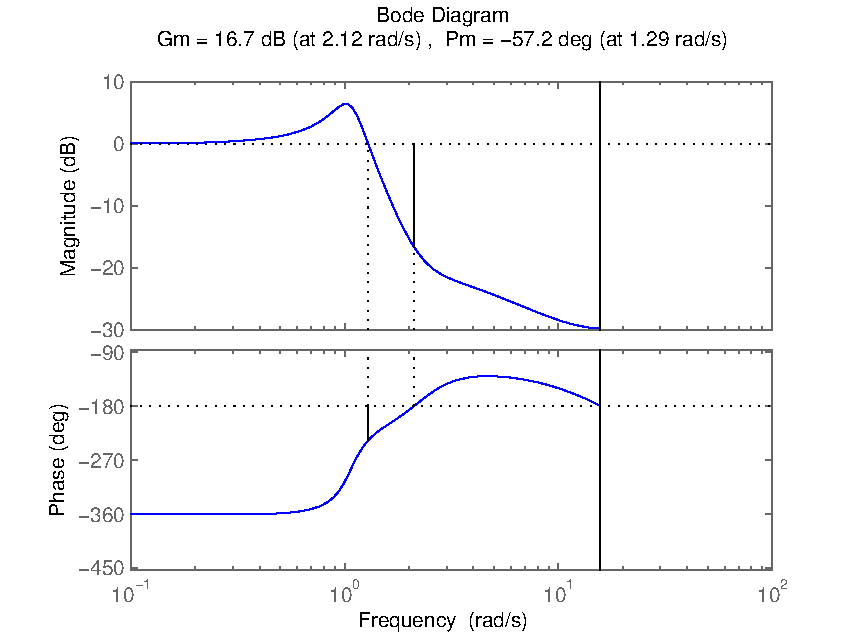
\includegraphics[width=\textwidth]{figures/runningexample_bd0.pdf}
        \caption{Original controller~\cite{DBLP:conf/hybrid/WangGRJF16}.}
        \label{fig:original}
    \end{subfigure}
    ~
    \begin{subfigure}[b]{0.4\textwidth}
        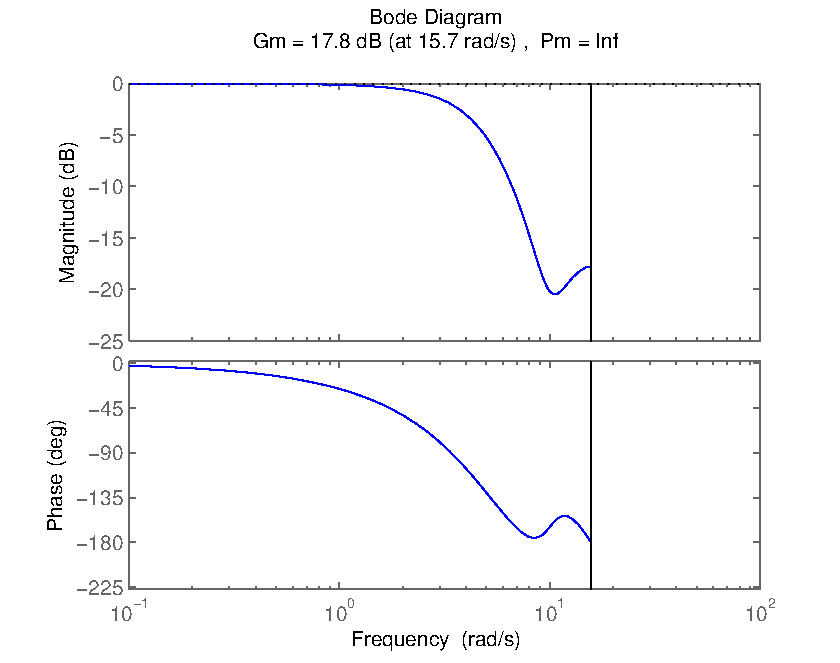
\includegraphics[width=\textwidth]{figures/runningexample_bd2.pdf}
        \caption{Controller synthesized by \tool.}
        \label{fig:cegiscontroller}
    \end{subfigure}
    \caption{Bode diagram for original~\cite{DBLP:conf/hybrid/WangGRJF16} and synthesized closed-loop systems.}\label{fig:bode}
\end{figure}

Figure~\ref{fig:step} illustrates the step responses of the closed-loop
system with the original controller represented by
Eq.~\eqref{Eq:running-example-controller} (Figure~\ref{fig:step0}), the
first (Figure~\ref{fig:step1}) and final (Figure~\ref{fig:step2}) candidate
solutions provided by \tool.  The step response in Figure~\ref{fig:step0}
confirms the stability loss if we consider FWL effects.  However,
Figure~\ref{fig:step1} shows that the first candidate controller is able to
stabilize the closed-loop system without uncertainties, but it is rejected
during the {\sc precision} phase by \tool since this solution is not
considered to be sound.  Finally, Figure~\ref{fig:step2} shows a stable
behavior for the final (sound) solution, which presents a lower settling
time.

\begin{figure*}
    \centering
    \begin{subfigure}[b]{0.3\textwidth}
        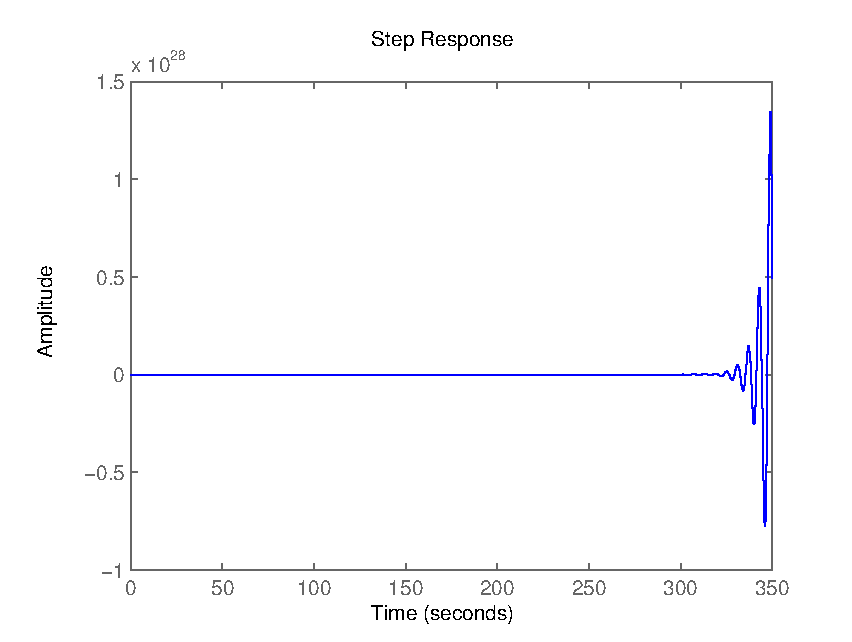
\includegraphics[width=\textwidth]{figures/runningexample_step0.pdf}
        \caption{Original controller}
        \label{fig:step0}
    \end{subfigure}
    ~
    \begin{subfigure}[b]{0.3\textwidth}
        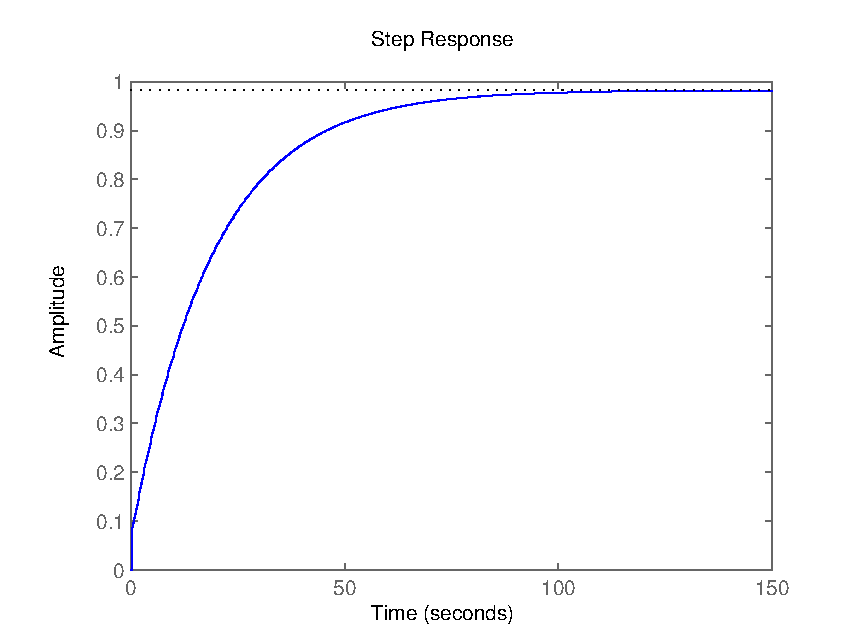
\includegraphics[width=\textwidth]{figures/runningexample_step1.pdf}
        \caption{First solution by \tool}
        \label{fig:step1}
    \end{subfigure}
    ~
    \begin{subfigure}[b]{0.3\textwidth}
        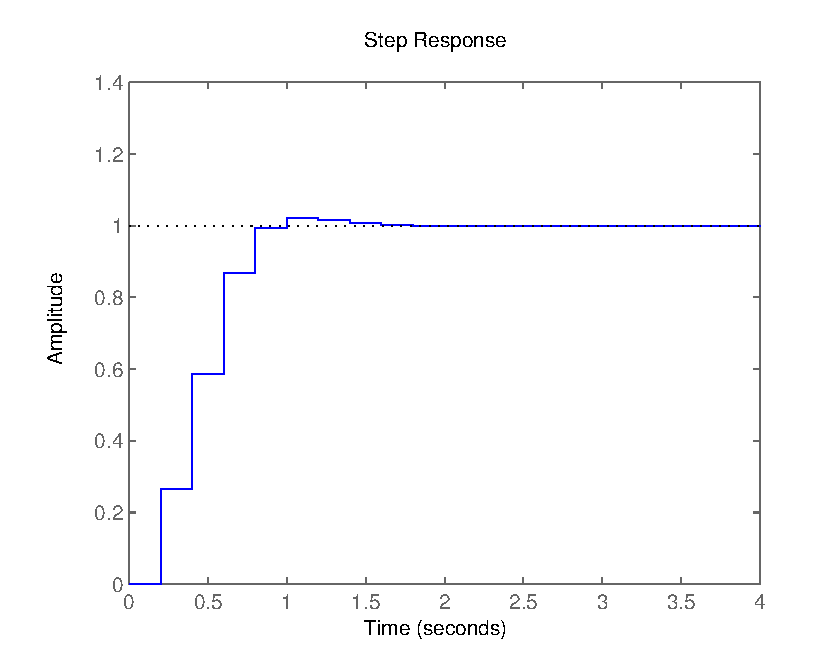
\includegraphics[width=\textwidth]{figures/runningexample_step2.pdf}
        \caption{Final solution by \tool}
        \label{fig:step2}
    \end{subfigure}
    \caption{Step responses for original~\cite{DBLP:conf/hybrid/WangGRJF16}
             closed-loop system with FWL effects and for each
             {\sc synthesize} iteration of \tool}\label{fig:step}
\end{figure*}

%%%%%%%%%%%%%%%%%%%%%%%%%%%%%%%%%%%%%%%%%%%%%%%%%%%%%%%%%%%%%%%%%%%%%%%%%%%%%%%%%%%%%%
\section{Experimental Evaluation}\label{sec:experiments}

This section is split into three parts. Section~\ref{experimental-setup}
discusses the experimental setup and our benchmarks, while
Section~\ref{experimental-objectives} describes the experimental objectives. 
Section~\ref{experimental-results} presents the experimental results
obtained on the benchmarks with our tool \tool.

%---------------------------------
\subsection{Description of the Benchmarks}
\label{experimental-setup}
%---------------------------------

The first set of benchmarks uses the discrete plant of a cruise control
model for a car, and accounts for rolling friction, aerodynamic drag, and
the gravitational disturbance force~\cite{Astrom08}. The plant model is
given as follows:
%
\begin{equation}
\label{cruise-control-c1}
G_1(z)=\frac{0.0264}{z-0.998} \nonumber
\end{equation} 

%Two proportional-integral (PI) controllers are designed by Wang {\it et al.} 
%for the cruise control plant $G(z)$~\cite{DBLP:conf/hybrid/WangGRJF16}, 
%which has the following mathematical model
%
%\begin{equation}
%\label{cruise-control-g1}
%C_{1}(z)=\frac{1.51z-1.3586}{z-1}, \nonumber
%\end{equation} 
%
%\begin{equation}
%\label{cruise-control-g2}
%C_{2}(z)=\frac{2.72z^2 - 4.153z + 1.896}{1.0z^2 - 1.844z + 0.8496}. \nonumber
%\end{equation} 

The second set of benchmarks considers a simple spring-mass 
damper~\cite{DBLP:conf/hybrid/WangGRJF16}, where the discrete 
plant dynamics is represented by the following $z$-expression:
%
%where both discrete 
%plant dynamics and controller are represented by the following 
%z-expression, resp.
%
\begin{equation}
\label{spring-mass-damper-g}
G_2(z)=\frac{5\times{10^{-5}}z + 5\times{10^{-5}}}{z^2 - 2z + 1.0001}. \nonumber
\end{equation} 
%
%\begin{equation}
%\label{spring-mass-damper-c}
%C_3(z)=\frac{1.28\times{10^{3}}z^2 - 1.354240\times{10^{3}}z + 0.074879\times{10^{3}}}{z^2 - 1.4990z + 0.4995}. \nonumber
%\end{equation} 

A third set of benchmarks uses a physical plant for satellite
applications~\cite{Franklin15}.  Satellites require attitude (pose) control
for orientation of antennas and sensors w.r.t.~earth.  The satellite
attitude control is typically used for three-axis attitude tracking, but
here we consider only one axis at a time.  The motion equation for the
one-axis system, disregarding disturbance torques, is given by
%
\begin{equation}
\label{eq:satelliteode}
I\cdot \ddot{\theta} = \tau_{C}, 
\end{equation}
%
\noindent where $I$ is the inertia moment of the satellite about its mass
center, $\tau_{C}$ is the control torque applied by the thrusters, and
$\theta$ is the controlled attitude angle.  Normalizing
Eq.~\eqref{eq:satelliteode} by defining the control signal
$u=\frac{\tau_{C}}{I}$ and taking the Laplace transform, the following
$s$-domain transfer function $G(s)$ is obtained:
%
\begin{equation}
\label{eq:satellitetf}
G_{3}(s)=\frac{\theta(s)}{u(s)}=\frac{1}{s^2},
\end{equation}
%
\noindent Using the ZOH discretization defined in Eq.~\eqref{eq:pulsetf}, 
we get the following $z$-domain model:
%
\begin{equation}
G_{3}(z)= \frac{T^{2}}{2} \frac{z+1}{(z+1)^{2}}. \nonumber
\end{equation}

%The discrete controllers $C_{4}$ and $C_{5}$ for the satellite plant $G_{3}$, discretized with sample time $1s$ and $2s$ respectively, 
%are represented by the following z-expression:
%
%\begin{equation}
%\label{satellite-b2}
%C_{4}(z)=\frac{2.88z^2 - 4.896z + 2.074}{1.0z^2 - 0.42z - 0.3465 - 0.03915}. \nonumber
%\end{equation} 
%
%\begin{equation}
%\label{satellite-c2}
%C_{5}(z)=\frac{0.43z^2 - 0.2408z - 0.1316}{1.0z^2 + 1.5z + 0.97 + 0.183}. \nonumber
%\end{equation} 

The fourth (and last) set of benchmarks considers the following description
for the plant $G_{4}(s)$, which is typically used for evaluating stability
margins~\cite{bhattacharyya97, keel_Bhattacharyya_examples}:
%
\begin{equation}
\label{exampleA}
G_{4}(s)=\frac{s-1}{s^{2}-s-2},
\end{equation}
%
\noindent We can obtain $G_{4}(z)$ using the ZOH discretization defined
in Eq.~\eqref{eq:pulsetf} with three different sample times ($0.1$, $0.05$,
and $0.03$ seconds), respectively, as follows:
%
\begin{equation}
\label{exampleA-sampletime1}
G_{4a}(z)=\frac{0.100342181002722z - 0.110876810062963}{1.0z^{2} - 2.12624017619613z + 1.10517091807565}, \nonumber
\end{equation}
%
%
\begin{equation}
\label{exampleA-sampletime2}
G_{4b}(z)=\frac{0.0500422033454653z - 0.0526068264456340}{1.0^{2} - 2.05640034257636z + 1.05127109637602}, \nonumber
\end{equation}
%
%
\begin{equation}
\label{exampleA-sampletime3}
G_{4c}(z)=\frac{0.0300090687252212z - 0.0309228417953966}{1.0^{2} - 2.03228208009387z + 1.03045453395352}. \nonumber
\end{equation}

All experiments were conducted on a 12-core 2.40\,GHz Intel Xeon E5-2440
with 96\,GB of RAM and Linux OS.  All times given are wall clock time in
seconds as measured by the UNIX date command.  For the approach using a
two-stage verification engine we apply a timeout of 8 hours per benchmark,
and 24 hours for the approach using a one-stage engine.

%---------------------------------
\subsection{Objectives}
\label{experimental-objectives}
%---------------------------------

Using the closed-loop control system benchmarks given in
Section~\ref{experimental-setup}, our experimental evaluation aims to answer
two research questions:
%
\begin{enumerate}

\item[RQ1] \textbf{(performance)} does the CEGIS approach generate a 
FWL digital controller in a reasonable amount of time?

\item[RQ2] \textbf{(sanity check)} are the synthesized controllers sound
and can their stability be confirmed outside of our model?

\end{enumerate}

%---------------------------------
\subsection{Results}
\label{experimental-results}
%---------------------------------

We give the runtimes required to synthesize a stable controller for each
benchmark in Table~\ref{tab:results}.  Here, \textit{Plant} is the discrete
or continuous plant model, \textit{Benchmark} is the name of the employed
benchmark, \textit{I} and \textit{F} represent the number of integer and
fractional bits of the stable controller, respectively, while \textit{Time}
is the total time (in seconds) required to synthesize a stable controller
for the given plant.

For the majority of our benchmarks, the conjecture explained in
Section~\ref{synthesis-elements} holds and the two-stage verification 
engine %inductive back-end 
is able to find a stable solution in less than five minutes.  This is possible if the
inductive solutions need to be refined with few counterexamples and
increases of the fixed-point precision.  However, two benchmarks in our set
required too many counterexamples to refine their solution (marked with $^*$
in Table~\ref{tab:results}).  In these cases, the one-stage engine 
%interval arithmetic back-end 
is able to complement the two-stage approach and synthesize a solution
instead, albeit with significantly larger runtimes.  This performance
difference is due to the fact that the one-stage verification engine does
not take advantage of the inductive conjecture inherent to CEGIS, but
instead fully explores the counterexample space.  The result is a
performance difference of at least two orders of magnitude in our
experiments, leading to the one-stage engine timing out on the majority of
our benchmarks.  Table~\ref{tab:results} only lists the faster of the two
verification engines for each benchmark, which in $12$ out of $15$
benchmarks is the two-stage one.

\begin{table}
\centering
\begin{tabular}{| r | c | l | r r || r | r |}
\hline
\# & Plant  & Benchmark                  & $I$ & $F$
   & 1-step & 2-step
    \\\hline\hline
1  & $G_1$  & CrsControl02
            &   4 &  16 & 17\,s   & \xmark     \\
2  & $G_1$  & CrsControl02$^\dagger$
            &   4 &  16 & 46\,s   & \xmark     \\
3  & $G_2$  & SpgMsDamper
            &  15 &  16 & 28\,s   & \xmark     \\
4  & $G_2$  & SpgMsDamper$^\dagger$
            &  15 &  16 & \xmark  & \xmark    \\
5  & $G_3$  & SatelliteB2
            &   3 &   7 & 7\,s    & \xmark     \\
6  & $G_3$  & SatelliteB2$^\dagger$
            &   3 &   7 & \xmark  & 6601\,s  \\
7  & $G_3$  & SatelliteC2
            &   3 &   5 & 2\,s    & \xmark    \\
8  & $G_3$  & SatelliteC2$^\dagger$
            &   3 &   5 & \xmark  & 76\,s    \\
9  & $G_4a$ & a\_ST1\_IMPL1
            &  16 &   4 & 2704\,s & \xmark   \\
10 & $G_4a$ & a\_ST1\_IMPL2
            &  16 &   8 & 538\,s  & \xmark   \\
11 & $G_4a$ & a\_ST1\_IMPL3
            &  16 &  12 & 12\,s   & \xmark   \\
12 & $G_4b$ & a\_ST2\_IMPL1
            &  16 &   4 & 318\,s  & \xmark   \\
13 & $G_4b$ & a\_ST2\_IMPL2
            &  16 &   8 & 967\,s  & \xmark    \\
14 & $G_4b$ & a\_ST2\_IMPL3
            &  16 &  12 & 9798\,s & \xmark   \\ 
15 & $G_4c$ & a\_ST3\_IMPL1
            &  16 &   4 & 6304\,s & \xmark   \\\hline
\end{tabular}

\vspace{0.5em}
\scriptsize{\xmark = time-out, $\dagger$ = with uncertainty}
\vspace{0.5em}

\caption{Experimental results obtained with \tool\label{tab:results}}
\end{table}
%---------------------------------

The median runtime for our benchmark set is $197$\,s, implying that \tool
can synthesize half of the controllers in less than $5$ minutes.  Overall,
the average synthesis time amounts to approximately $30$ minutes.  We
consider these times short enough to be of practical use to control
engineers, and thus affirm RQ1.  We further observe that the approach using
the two-stage verification engine is able to synthesize stable controllers
in $12$ out of the $15$ benchmarks, and can be complemented using the
one-stage engine for two additional benchmarks, where the inductive
conjectures fail.  Both verification engines together enable controller
synthesis for $14$ out of $15$ benchmarks.  For the one remaining benchmark
our approach failed to synthesize a stable controller within the time
limits.  This can be addressed by either increasing the fixed-point word
widths considered or using floating-point arithmetic instead.  The
synthesized controllers were confirmed to be stable outside of our model
representation using MATLAB, positively answering RQ2.  A~link to the full
experimental environment, including scripts to reproduce the results, all
benchmarks and the \tool tool, is provided in the
footnote.\footnote{\url{https://drive.google.com/file/d/0ByIexo3Z5N91QkhrMi1rdkZFTWc/view}}

\subsection{Threats to validity}

We report a favourable assessment of \tool over a diverse set of real-world
benchmarks. Nevertheless, this set of benchmarks is limited within the
scope of this paper and \tool's performance may not generalize to other
benchmark scenarios. This can be addressed by expanding the benchmark set
in future experiments.

Furthermore, our algorithm to select suitable FWL word widths to model
plant behavior employs a heuristic based on user-provided controller
word-width specifications.  Given the encouraging results of our benchmarks,
this heuristic appears to be strong enough for the current benchmark set,
but this may not generalize.  Further experiments towards determining
suitable plant FWL configurations may thus be necessary in future work.

Finally, the experimental results obtained using \tool for stability
properties may not generalize to other properties.  The inductive nature of
the two-stage back-end of \tool increases performance significantly compared
to the one-stage back-end, but this performance benefit introduced by CEGIS'
inductive generalizations may not be observed for other controller
properties.  Additional experiments are necessary to confirm that the
performance of our inductive synthesis approach can be leveraged in those
scenarios as well.

%%%%%%%%%%%%%%%%%%%%%%%%%%%%%%%%%%%%%%%%%%%%%%%%%%%%%%%%%%%%%%%%%%%%%%%%%%%%%%%%%%%%%%
\section{Related Work}\label{sec:related}

\paragraph{Robust synthesis of Linear Systems} 

The problem of parametric control synthesis based on stability measures for
continuous Linear Time Invariant (LTI) Single Input-Single Output (SISO)
systems has been researched for several decades.  On a theoretical level it
is a solved problem~\cite{wonham1967pole}, for which researchers
continuously seek better results for a number of aspects in addition to
stability.  A vast range of pole placement techniques such as Moore's
algorithm for eigenstructure assignment~\cite{klein1977eigenvalue} or the
more recent Linear Quadratic Regulator (LQR)~\cite{bemporad2002explicit}
have been used in several studies with increasing degrees of success to
ensure stability.  The latter approach highlights the importance of
conserving energy during the control process, which results in lower running
costs.  Since real systems are subject to tolerance and noise as well as the
need for economy, more recent studies focus on the problem of achieving
robust stability with minimum gain~\cite{schmid2014unified,
konigorski2012pole}.  However, when applied with the aim of synthesising a
digital controller, many of these techniques lack the ability to produce
sound or stable results because they disregard the effects of quantization
and rounding.  Recent papers on implementations/synthesis of LTI digital
controllers~\cite{das2013lqr, ghosh2013fpga} focus on time discretization,
failing to account for these error-inducing effects and can therefore result
in digital systems that are unstable even though they have been proven to be
robustly stable in a continuous space.  

\paragraph{Formal Verification of Linear Digital Controllers} 

Researchers in formal verification of control systems have studied various
effects of discretizing the dynamics, including delayed
response~\cite{Duggirala2015}, and Finite Word Length (FWL) semantics with
the goal to either verify (e.g.~\cite{daes20161}) or optimize
(e.g.~\cite{oudjida2014design}) given implementations.

There are two different problems that arise from FWL semantics.  The first
is the error in the dynamics caused by the inability to represent the exact
state of the physical system while the second relates to rounding errors
during computation.  In~\cite{fialho1994stability}, a stability measure
based on the error of the digital dynamics ensures that the deviation
introduced by FWL does not make the digital system unstable.  A more recent
approach~\cite{DBLP:journals/automatica/WuLCC09} uses the $\mu$-calculus to
directly model the digital controller so that the selected parameters are
stable by design.  Most work in verification focusses on finding a correct
variant of a known controller, e.g., by looking for optimal parameter
representations using FWL, but ignore the effects of rounding errors due to
issues of mathematical tractability.  The analyses
in~\cite{DBLP:conf/hybrid/WangGRJF16, DBLP:conf/hybrid/RouxJG15} rely on an
invariant computation on the discrete system dynamics using Semi-Definite
Programming (SDP).  While the former uses BIBO properties to determine
stability, the latter uses Lyapunov-based quadratic invariants.  In both
cases, the SDP solver uses floating-point arithmetic and soundness is
checked by bounding the error.  An alternative approach is taken
by~\cite{park2016scalable}, where the verification of existing code is
performed against a known model by extracting an LTI model of the code
through symbolic execution.  In order to account for rounding errors, an
upper bound is introduced in the verification phase.  If~the error of the
implementation is lower than this tolerance level, then the verification is
successful.

\paragraph{Robust Synthesis of FWL Digital Controllers}

There is no technique in the existing literature for automatic synthesis of
fixed-point digital controllers that considers FWL effects.  Parameter
synthesis tools such as~\cite{cimatti2013parameter} use bounded model
checking and fixed-point computations to compute parameters based on
user-defined specifications, but they often operate in the continuous domain
and have no direct means of evaluating robustness.

Other tools such as~\cite{economakos2016automated} are directly aimed at
robust stability problems, but they fail to take the effects of FWL into
account.  In order to provide a correct-by-design digital controller,
\cite{alur2016compositional} requires a user-defined finite-state
abstraction to synthesize a digital controller based on high-level
specifications.  While this approach overcomes the challenges presented by
the FWL problem, it still requires error-prone user intervention. 
A~different solution that uses FWL as the starting point is an approach that
synthesizes word lengths for known control problems~\cite{jha2013swati};
however, this provides neither an optimal result nor a comprehensive
solution for the problem.

\paragraph{CEGIS}

Program synthesis is the problem of computing correct-by-design programs
from high-level specifications, and algorithms for this problem have made
substantial progress in recent years.  One such
approach~\cite{itzhaky2010simple} inductively synthesizes invariants to
generate the desired programs.

Program synthesisers are an ideal fit for synthesis of parametric
controllers since the semantics of programs capture effects such as FWL
precisely.  In~\cite{DBLP:conf/cdc/RavanbakhshS15}, the authors use CEGIS
for the synthesis of switching controllers for stabilizing continuous-time
plants with polynomial dynamics.  The work extends to its application on
affine systems, finding its major challenge in the hardness of solving
linear arithmetic with the state-of-the-art SMT solvers.  Since this
approach uses switching states instead of linear dynamics in the digital
controller, it entirely circumvents the FWL problem.  It is also not
suitable for the kind of control we seek to synthesize.  We require a
combination of a synthesis engine with a control verification tool that
addresses the challenges presented here in the form of FWL effects and
stability measures for LTI SISO controllers.  We take the former
from~\cite{DBLP:conf/lpar/DavidKL15} and the latter from~\cite{daes20161}
while enhancing the procedure by evaluating the quantization effects of the
Hardware interfaces (ADC/DAC) to obtain an accurate discrete-time FWL
representation of the continuous dynamics.
 
%In \cite{DBLP:journals/corr/PakmehrWJVF13}, Pakmehr et al.  design a control software verification framework for gas turbine engines.

%%%%%%%%%%%%%%%%%%%%%%%%%%%%%%%%%%%%%%%%%%%%%%%%%%%%%%%%%%%%%%%%%%%%%%%%%%%%%%%%%%%%%%
\section{Conclusions} \label{sec:conclusions}

We have presented a CEGIS-based approach implemented in a tool called \tool,
which uses inductive synthesis in conjunction with an algorithm for
verifying robust closed-loop stability.  In particular, \tool is able to
compute a parametric solution for a stabilizing digital controller given a
continuous (or discrete) plant specification.  This enables us to
automatically synthesize correct-by-construction digital controllers for a
given model of their physical environment.  Our approach addresses the
effects of the quantizers (A/D and D/A converters) as time discretization
elements with quantization noise.  Our experimental results show that \tool
is able to synthesize stable controllers in most benchmarks within
a reasonable amount of time fully automatically.
%
% and can be 
%complemented using the interval arithmetic back-end, where the inductive conjectures fail. 
%Both back-ends enabled controller synthesis for all benchmarks within reasonable time frames.

Future work will be the extension of this CEGIS-based approach to further
classes of systems, including state-space representation.  We will also
consider performance requirements while synthesizing the digital controller.

\bibliographystyle{abbrv}
\bibliography{paper}  

%APPENDICES are optional
%\balancecolumns
%\appendix
%Appendix A

\end{document}
